\chapter{}

\section{A Picture of Nuclear Matter}
\label{sec:nuclear_matter}

%\textcolor{red}{Missing bridge from QCD to hadrons.}

%\textcolor{red}{[Part of it may migrate. At some point before, introduce the proton as something more than 3 quarks]}

Probing hadrons at high energies in scattering experiments has allowed exploring the internal structure of nucleons. Data from  both fixed-target and collider (\gls{HERA}, Tevatron, \gls{LHC}) experiments has been compiled in order to obtain pictures of the gluon and quark content of hadrons. In this context, one may refer collectively to quarks and gluons as partons.

At \gls{HERA}, electrons (or positrons) and protons were accelerated to collide at center of mass energies of around $\sqrt{s} = \qty{300}{GeV}$. In some of these collisions, the momentum transfer $Q^\mu$ from the electron to the proton via a virtual photon was large enough ($Q^2 > \qty{200}{GeV^2}$) to disintegrate the proton into a shower of hadrons $(e  + p \to e + X)$; these are called \gls{DIS} processes, whose cross-sections are valuable in unveiling the proton's parton content. The greater the virtual photon's energy, the greater its ability to resolve structures of smaller scale than the proton radius and with shorter characteristic timescales, since the spatial and temporal resolutions of these experiments are roughly proportional to $1/Q$.
% or $1/\sqrt{s}$.
 \gls{DIS} processes have also been studied for this purpose using muons and neutrinos as probes, and neutrons as targets -- each probe selects for different processes of interaction with the hadron, which allow assessing the abundance of different, specific species of partons\footnote{For example, the use of neutrinos as probes permits scanning for $\nu + N \to \mu^- + X$ (with $N$ a nucleon) events, where it is guaranteed that a $W^+$ boson was exchanged between the neutrino and a negatively charged quark or antiquark.}; using the neutron as a target also provides insight into the internal structure of the proton due to their similarity: in the static quark model, the quark compositions of the proton and the neutron are uud and ddu. At the Tevatron and LHC colliders, data from $p\overline{p}$ and $pp$ collisions, respectively, has contributed to the study of the gluon content of protons, specifically. \cite{Thomson8:2013,PDG_2024} Unlike at HERA, in these experiments the two projectiles may exchange a virtual color-charged particle, which allows for processes useful in assessing the abundance of gluons without interference from the quark content. \cite[Table 18.1]{PDG_2024}
%is capable of interacting with the projectiles' constituent gluons.

The contributions from these many experiments have permitted the quantitative assessment of the proton's parton content via the measurement of its \glspl{PDF}. These translate the abundance, inside the proton, of a given parton species carrying a certain fraction of its momentum (in a frame of reference where the proton's momentum is large). A species $q$'s \gls{PDF}, $q(x)$, is defined such that the number of $q$ partons carrying a fraction of the proton's momentum between $x$ and $x + \Delta x$, in a frame where the proton's momentum is much greater than its mass, is given by $q(x)\Delta x$. These functions actually also depend on the energy scale of the process used to probe the proton, $Q^2$, since a greater exchange of energy allows probing finer features of the proton, increasing its \glspl{PDF} at small $x$, for example. \cite{Thomson8:2013}

Fig. \ref{fig:PDFs} shows a recent result for the proton's \glspl{PDF}. For $0.1 \lesssim x < 1$, the ``valence" quarks $u$ ($\mathbf{u}_V$) and $d$  ($\mathbf{d}_V$) dominate, and in the relative proportion expected from the static quark model, $uud$. However, for $x \lesssim 0.02$, they are overtaken by a ``sea" of quarks and antiquarks. These may be thought of as $q\overline{q}$ pairs arising from interactions between the valence quarks. Therefore, any ``sea'' flavor's \gls{PDF} is identical to its antiquark's \gls{PDF}. The ``sea'' includes new flavors ($s$, $c$ and $b$) and $u$ and $d$ quarks which are as abundant as the $\overline{u}$ and $\overline{d}$ antiquarks; to distinguish them from their valence counterparts, their \glspl{PDF} are written $\mathbf{\overline{u}}$ and $\overline{\mathbf{d}}$. For small $x$, however, the most abundant parton is, by far, the gluon ($\mathbf{g}$).

\begin{figure}[h]
    \centering
    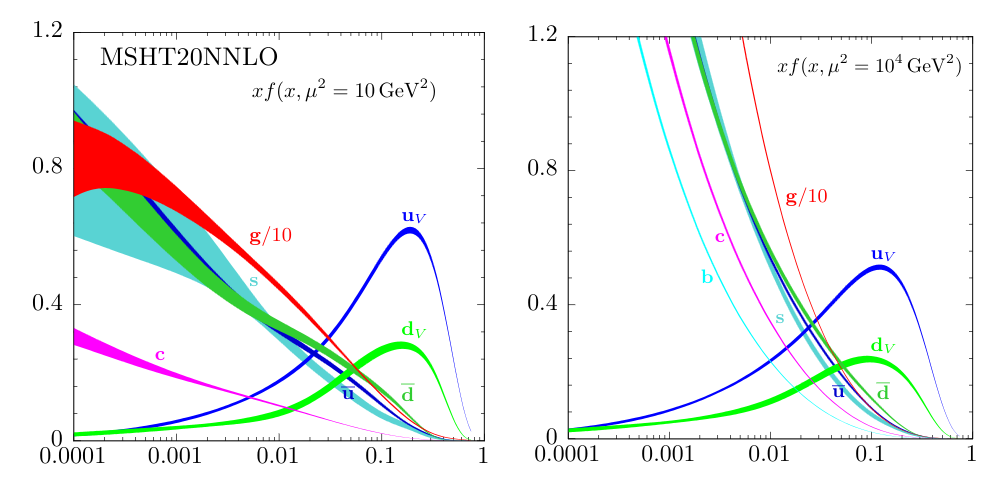
\includegraphics[width=\textwidth]{Figures/PDFs_2021.png}
    \caption[The proton's \glshyperlink{PDF}s multiplied by $x$ calculated at \glshyperlink{NNLO} for the case of unpolarized beams at the energy scales $\mu^2 = \qty{10}{GeV^2}$ (left) and $\mu^2 = 10^4\qty{}{GeV^2}$ (right). The gluon's \glsentryfirst{PDF} appears scaled down by a factor of 10. \cite{PDG_2024} Originally from and calculated by the MSHT Group in 2020. \cite{Bailey_2021}]{The proton's \glspl{PDF} multiplied by $x$ calculated at \gls{NNLO} for the case of unpolarized beams at the energy scales $\mu^2 = \qty{10}{GeV^2}$ (left) and $\mu^2 = 10^4\qty{}{GeV^2}$ (right). The gluon's \gls{PDF} appears scaled down by a factor of 10. \cite{PDG_2024} Originally from and calculated by the MSHT Group in 2020. \cite{Bailey_2021}}
    \label{fig:PDFs}
\end{figure}

\section{Gluon Saturation}
\label{sec:gluon_saturation}

%\textcolor{red}{[Missing a discussion of evolution in $Q$ (DGLAP) vs evolution in $x$ (BFKL) accompanied by the usual $x$ vs. $Q$ plot -- should include "linear evolution predicts exponential growth.]}
%\textcolor{red}{[Refer previous discussion of low-$x$ gluon abundance]}

The dominance by the gluon over the proton's parton content  at low-$x$ is predicted by \gls{QCD}. Two avenues for reaching this prediction will be explored in this section: first, using the splitting function of the gluon and, second, using the \gls{QCD} evolution equations.
\textcolor{purple}{$\times$}%since the fits that obtain fid 1's pdfs include the DGLAP (and BFKL?) equations, this feels a bit dishonest, maybe?

The splitting function of non-Abelian gauge bosons such as the gluon is a well know \gls{QCD} result. It returns the probability of emission by a parton of a gluon with relative transverse momentum $\mathbf{k}_\perp$ and a fraction $x$ of its longitudinal momentum. In the soft limit, at lowest order in $\alpha_S$ and for small $x$, it reads \cite{Gelis_2010}:
\begin{equation}
	\diff P \propto \frac{\alpha_S}{\pi^2} \frac{\diff^2 \mathbf{k}_\perp}{|\mathbf{k}_\perp|^2} \frac{\diff x}{x}
\end{equation}
The probability then contains colinear ($|\mathbf{k}|_\perp \to 0$) and soft ($x \to 0$) logarithmic singularities. The singularity as $x \to 0$ suggests a picture of abundance of small-$x$ gluons within all hadrons, which grows uncapped as partons emit small-$x$ gluons, which themselves emit smaller-$x$ gluons or produce quark-antiquark pairs which also serve as gluon emitters. However, gluon densities may not explode as $x \to 0$, otherwise, unitarity would be violated. \cite{Albacete_2014}

Below a certain value of $x$, non-linear dynamics not considered so far should take over and tame the divergence, \textit{saturating} the low-$x$ gluon density in the hadron. The onset of saturation is controlled by the saturation scale, $Q_s(x)$, a transverse momentum scale below which non-linear effects become relevant. \cite{Albacete_2014}

One interpretation of these non-linear effects is the onset, above certain gluon densities, of gluon recombination. Above that threshold, the probability of emission of a new gluon becomes comparable to the probability of recombination of gluons, slowing the growth of their density to rates compatible with conservation of unitarity (Fig. \ref{fig:gluon_recombination}).
%\begin{figure}[h]
%    \centering
%    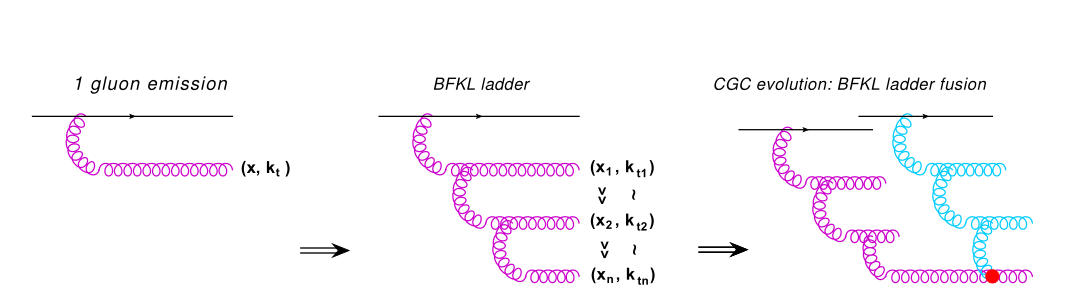
\includegraphics[width=\textwidth]{Figures/gluon_recombination.png}
%    \caption{The onset of gluon recombination. Above a certain gluon density, gluon recombination (red dot) becomes comparatively likely to gluon emission (the pink and blue ladders of gluons). Taken from \cite{Albacete_2014}.}
%    \label{xxx}
%\end{figure}
\begin{figure}[h]
    \centering
    %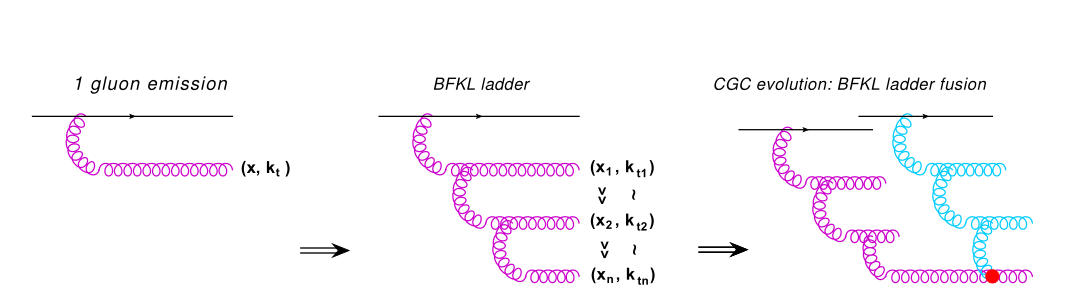
\includegraphics[width=\textwidth]{Figures/gluon_recombination.png}
    \begin{equation*}
\begin{tikzpicture}[baseline=(g12.base)]
\begin{feynman}[inline=g12.base)]
\vertex (q1);
\vertex[right=0.7cm of q1] (q2);
\vertex[right=3cm of q1] (q3);
\vertex[below=0.8cm of q2] (g11);
\vertex[below=0.8cm of q3] (g12);
%\vertex at ($(a1)!0.5!(b1)$) (ctr);
\diagram* {
(q1) -- [fermion] (q3),
(q2) -- [gluon, half right,magenta] (g11),
(g11) -- [gluon,magenta] (g12),
};
\end{feynman}
\end{tikzpicture}
\quad \to \quad
\begin{tikzpicture}[baseline=(g13.base)]
\begin{feynman}[inline=g13.base)]
\vertex (q1);
\vertex[right=0.7cm of q1] (q2);
\vertex[right=3cm of q1] (q3);

\vertex[below=0.8cm of q2] (g11);
\vertex[right=0.7cm of g11] (g12);
\vertex[below=0.8cm of q3] (g13);
\vertex[right=0.1cm of g13] (g13l) {$x_1$};

\vertex[below=0.8cm of g12] (g21);
\vertex[right=0.7cm of g21] (g22);
\vertex[below=0.8cm of g13] (g23);
\vertex[right=0.1cm of g23] (g23l) {$x_2$};

\vertex[below=0.8cm of g22] (g31);
\vertex[below=0.8cm of g23] (g32);
\vertex[right=0.1cm of g32] (g32l) {$x_3$};

\vertex at ($(g13l)!0.5!(g23l)$)[rotate=270] (gg1) {$\gg$};
\vertex at ($(g23l)!0.5!(g32l)$)[rotate=270] (gg2) {$\gg$};

%\vertex at ($(a1)!0.5!(b1)$) (ctr);
\diagram* {
(q1) -- [fermion] (q3),
{[edges=gluon]
(q2) -- [half right,magenta] (g11) -- [magenta] (g12) -- [magenta] (g13),
(g12) -- [half right,magenta] (g21) -- [magenta] (g22) -- [magenta] (g23),
(g22) -- [half right,magenta] (g31) -- [magenta] (g32),
},
};
\end{feynman}
\end{tikzpicture}
\quad \to \quad
\begin{tikzpicture}[baseline=(g13.base)]
\begin{feynman}[inline=g13.base)]
\vertex (q1);
\vertex[right=0.7cm of q1] (q2);
\vertex[right=3cm of q1] (q3);

\vertex[below=0.8cm of q2] (g11);
\vertex[right=0.7cm of g11] (g12);
\vertex[below=0.8cm of q3] (g13);

\vertex[below=0.8cm of g12] (g21);
\vertex[right=0.7cm of g21] (g22);
\vertex[below=0.8cm of g13] (g23);

\vertex[below=0.8cm of g22] (g31);
\vertex[right=3cm of g31,circle,fill=red] (g32) {};
\vertex[right=0.9cm of g32] (g33);
%%%%%%%%%%%%%%%%%%%%%%%%%%%%%%%%%%%
\vertex[right=3cm of q1] (peq1);
\vertex[above=0.3cm of peq1] (eq1);
\vertex[right=0.7cm of eq1] (eq2);
\vertex[right=3cm of eq1] (eq3);

\vertex[below=0.8cm of eq2] (eg11);
\vertex[right=0.7cm of eg11] (eg12);
\vertex[below=0.8cm of eq3] (eg13);

\vertex[below=0.8cm of eg12] (eg21);
\vertex[right=0.7cm of eg21] (eg22);
\vertex[below=0.8cm of eg13] (eg23);

\vertex[below=0.8cm of eg22] (eg31);
\vertex[below=0.8cm of eg23] (eg32);

%\vertex at ($(a1)!0.5!(b1)$) (ctr);
\diagram* {
(q1) -- [fermion] (q3),
{[edges=gluon]
(q2) -- [half right,magenta] (g11) -- [magenta] (g12) -- [magenta] (g13),
(g12) -- [half right,magenta] (g21) -- [magenta] (g22) -- [magenta] (g23),
(g22) -- [half right,magenta] (g31) -- [magenta] (g32) -- [magenta] (g33),
},

(eq1) -- [fermion] (eq3),
{[edges=gluon]
(eq2) -- [half right,cyan] (eg11) -- [cyan] (eg12) -- [cyan] (eg13),
(eg12) -- [half right,cyan] (eg21) -- [cyan] (eg22) -- [cyan] (eg23),
(eg22) -- [half right,cyan] (g32),
},
};
\end{feynman}
\end{tikzpicture}
\end{equation*}
    \caption{The onset of gluon recombination. Above a certain gluon density, gluon recombination (red dot) becomes comparatively likely to gluon emission (the pink and blue ladders of gluons). Adapted from \cite{Albacete_2014}.}
    \label{fig:gluon_recombination}
\end{figure}

\medskip
An uncapped growth of gluon densities in the proton is also quantitatively predicted by the evolution equations of \gls{QCD}. These perturbative equations provide a picture of how the parton content of the proton should evolve with $x$ and with the energy scale, $\mu$. %The \gls{BFKL} equations, specifically, quantitatively predict the growth of gluon densities at low-$x$.

The \gls{DGLAP} differential equation describes how \glspl{PDF} should evolve with $\mu$ at fixed $x$. They predict that all partons' \glspl{PDF} at low-$x$ should grow when $\mu$ is increased, as in Fig. \ref{fig:PDFs}. \cite{Halzen:1984mc}\footnote{In this book the \gls{DGLAP} equations are referred to as the Altarelli-Parisi equations.} The \glspl{PDF} of the valence quarks, specifically, grow at low-$x$ and shrink at high-$x$ when $\mu$ is increased, effectively moving them back along the $x$ axis. This reflects the fact that increasing the energy of the probing process allows resolving lower energy partons in the proton -- low-$x$ gluons emitted by a valence quark may be distinguishable at a higher $\mu$ but seen as part of the valence quark at a lower $\mu$ (Fig. \ref{fig:DGLAP_resolution}).
%\begin{figure}[h]
%    \centering
%    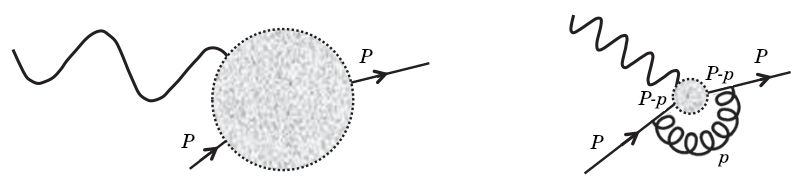
\includegraphics[width=\textwidth]{Figures/DGLAP_resolution.png}
%    \caption{.}
%    \label{fig:DGLAP_resolution}
%\end{figure}
\begin{figure}[h]
    \centering
    \begin{minipage}[c]{0.4\textwidth}
    \centering 
\begin{tikzpicture}%[baseline=(ctr.base)]
\begin{feynman}[large]%[inline=ctr.base)]
\vertex (c);
\vertex[above left= of c] (p);
\vertex[below left= of c] (q1);
\vertex[right= of c] (q2);

\diagram* {
(q1) -- [fermion, momentum=\(P\)] c [blob,minimum height=1.8cm, minimum width=1.8cm] -- [fermion] (q2),
(p) -- [yourboson] c,
};
\end{feynman}
\end{tikzpicture}
\end{minipage}
\begin{minipage}[c]{0.4\textwidth}
    \centering 
\begin{tikzpicture}%[baseline=(ctr.base)]
\begin{feynman}[large]%[inline=ctr.base)]
\vertex (c);
\vertex[above left= of c] (p);
\vertex[below left= of c] (q1);
\vertex[right= of c] (q2);

\vertex at ($(q1)!0.6!(c)$) (q11);
\vertex at ($(q2)!0.6!(c)$) (q22);

\diagram* {
(q1) -- [fermion, momentum=\(P\)] (q11) -- [plain, momentum=\(P-q\)] c [blob,minimum height=0.5cm, minimum width=0.5cm] -- [plain] (q22) -- [fermion] (q2),
(p) -- [photon] (c),
(q11) -- [gluon, half right, momentum' = \(q\)] (q22),
};
\end{feynman}
\end{tikzpicture}
\end{minipage}
    \caption{(Left) A quark being resolved as having momentum $P$ by a low-energy photon. (Right) The same quark becoming distinguishable from a gluon it emitted when probed by a high-energy photon, which resolves it as having momentum $P-q$. Adapted from \cite{Thomson:2013}.}
    \label{fig:DGLAP_resolution}
\end{figure}

The \gls{BFKL} differential equations, on the other hand, describe how gluon density in momentum space, $\phi$, should evolve with $x$ at fixed $\mu$. It is a linear equation, and predicts
%an exponential growth of the gluon density with rapidity, Y = ln(1/x); equivalently, it predicts
a divergence of the gluon density as $x \to 0$; more specifically, it predicts an exponential growth of $\phi$ with rapidity, $y \equiv \ln(1/x)$. The equation does not contain any terms reflecting interference between gluon emitters, as it assumes the hadron to be a dilute parton system. However, making the probability of emission of a new gluon dependent on the present gluon density by adding non-linear terms to the \gls{BFKL} equations allows for saturation to be reached when gluon generation and gluon recombination balance out. These new non-linear terms have coefficients that are inverse powers of energy scales, $(1/Q)^n$; they control when the new terms become comparable to the old linear terms, and thus act as saturation scales, $Q_s$. \cite{Albacete_2014}

Figure \ref{fig:DGLAPvsBFKL} illustrates the evolution of the parton content of the proton when its characterizing functions are evolved via the \gls{DGLAP} and the \gls{BFKL} equations. The upper left corner of this plot corresponds to the saturation region, where non-linear effects like recombination are thought to take over, otherwise gluon density growth as $x\to 0$ would violate unitarity.
%QCD evolution equations which attempt to incorporate this effect have additional, non-linear, density-dependent terms, such as the \gls{GRL-MQ} equation.
\begin{figure}[h]
    \centering
    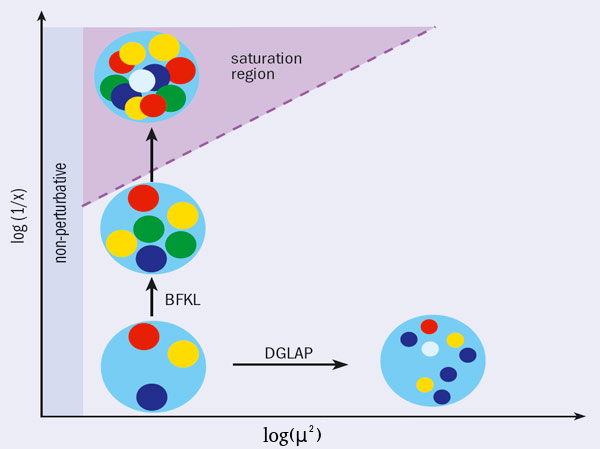
\includegraphics[width=0.6\textwidth]{Figures/DGLAPvsBFKL.png}
    \caption{An energy scale, $\mu$, vs. $x$ plot illustrating the evolution of the parton content of the proton via the \gls{DGLAP} and \gls{BFKL} equations. Moving left to right via \gls{DGLAP}, parton populations increase but the circles representing them get smaller, reflecting the decreasing characteristic length scale of the probing process ($\sim 1/\mu$). Moving bottom to top via \gls{BFKL}, parton populations also increase but the partons' size remains the same; the region where there are enough partons to force the circles to overlap is used as an analog for the region of this phase space where the proton should become saturated -- an area of interest for exploration in collider experiments.  Adapted from \cite{Diakonov2010}.}
    \label{fig:DGLAPvsBFKL} %does it make a difference to move horizontally first and then vertically or vice-versa?
\end{figure}


%More formally, the \gls{BFKL} \gls{QCD} evolution equation is a linear differential equation that governs how gluon density in momentum space within a hadron should evolve with $x$ when that hadron is probed at a fixed energy scale ($\mu^2$ is constant). It is a linear equation, and it predicts
%an exponential growth of the gluon density with rapidity, Y = ln(1/x); equivalently, it predicts
%a divergence of the gluon density as $x \to 0$. The equation does not contain terms reflecting interference between emitters of gluons, as it assumes the hadron to be a dilute parton system. However, making the probability of emission of a new gluon dependent on the present gluon density allows for saturation to be reached when gluon generation and gluon recombination balance out. QCD evolution equations which attempt to incorporate this effect have additional, non-linear, density-dependent terms, such as the \gls{GRL-MQ} equation. \cite{Albacete_2014}

The proton's (and, therefore, the heavy ion's) content may thus be thought of as dominated by its saturated low-$x$ gluon population. Over the next sections, a formalism for handling systems like this, the \gls{CGC}, \glsreset{CGC} will be introduced, preceded by a review of the \gls{QCD} Lagrangian and the definition of a practical set of coordinates in the context of a \gls{HIC}.

\section{The QCD Lagrangian}

In studying a system where strong interactions are dominant, one turns to the QCD Lagrangian, which encodes those interactions. It is a functional of the quark fields, $\psi$, which are 4-component Dirac spinors (with $\overline{\psi} = \psi^\dagger \gamma^0$ being the quark field's Dirac adjoint), and of the gluon fields (also called color fields), $A^a_\mu$, which are real-valued four-vectors; both are functions of spacetime. For a theory with $N_c$ colors and $N_f$ flavors of quarks each with mass $m_f$,
% in the presence of external color charge sources $J^\mu (x)$,
 the Lagrangian is
\begin{equation}
	\mathcal{L}_\text{QCD} = \sum_{f=1}^{N_f}\overline{\psi}_f \left(i \gamma^\mu D_\mu - m_f \right) \psi_f - \frac{1}{2} \Tr_c \left[ F_{\mu \nu} F^{\mu \nu} \right] %\textcolor{blue}{-2 \Tr [A_\mu J^\mu]}
	\label{eq:QCD_Lagrangian}
\end{equation}
where $D_\mu$, the covariant derivative, is given by:
\begin{equation}
	D_\mu =  \partial_\mu + i g A_\mu, \quad \text{where }  A_\mu = A_\mu^a T_a
\end{equation}
and $F^{\mu \nu}$, the gluon field strength tensor, is given by:
\begin{equation}
\begin{split}
	F_{\mu \nu} &\equiv F_{\mu \nu}^a T_a\\
	F_{\mu \nu}^a & = \partial_\mu A_\nu^a - \partial_\nu A_\mu^a - g f^{a b c} A^b_\mu A^c_\nu
\end{split}
\end{equation}
% = \partial_\mu A_\nu - \partial_\nu A_\mu + ig [A_\mu, A_\nu]
%\textcolor{blue}{and $J_\mu$, similarly to $A_\mu$, is a four-vector and  a linear combination of the $T_a$:
%\begin{equation}
%	J_\mu \equiv J_\mu^a T^a
%\end{equation}}
where $g$ is the Strong Force's coupling constant; $T^a$ are the SU($N_c$) generators in the fundamental representation\footnote{Normalized such that $\Tr_c [T^a, T^b] = \delta^{ab}/2$}, and $f^{abc}$ are the SU($N_c$) structure constants. $\Tr_c$ denotes a color-trace, that is, a trace in color space, the space of the $T_a$ matrices' indices.

%where the 4-component Dirac spinor $\psi$ is the quark field, a function of spacetime; $\overline{\psi}$ is its Dirac adjoint, $ \psi^\dagger \gamma^0$; $m$ is that quark flavour's mass; $D^\mu$ is the covariant derivative, obtained from the four-vector $A^\mu$, which is in turn obtained from a linear combination of the SU($N_c$) generators in the fundamental representation, $T^a$, with the real-valued gluon fields $A_\mu^a$, functions of spacetime, serving as coefficients; $F^{\mu \nu}$ is called the gluon field strength tensor; and $\Tr_c$ denotes a color-trace, that is, a trace in color space, where the $T_a$ live.

Writing the Lagrangian with all indices explicit,
\begin{equation}
	\mathcal{L}_{\text{QCD}} =  \sum_{f=1}^{N_f} \left(\psi_{\alpha f}^i \right)^*  \left( \gamma^0  \right)_{\alpha \beta} \left(i \left(\gamma^\mu \right)_{\beta \gamma} \left( \delta^{ij} \partial_\mu - i g A^a_\mu \left( T^a \right)^{ij} \right) - \delta_{\beta \gamma} \delta^{ij} m_f \right) \psi_{\gamma f}^j - \frac{1}{4} F_{\mu \nu}^a F^{\mu \nu}_a
	%\textcolor{blue}{- A_\mu^a J^\mu_a}
	\label{eq:QCD_Lagrangian_Indices}
\end{equation}
where $\alpha, \beta, \gamma = 1,2,3,4$ are Dirac indices, $i,j=1, ..., N_c$ are color indices in the fundamental representation, $a = 1, ..., {N_c}^2-1$ are color indices in the adjoint representation, $f = 1, ..., N_f$ are flavor indices and $\mu,\nu = 0,1,2,3$ are spacetime indices when using Minkowski coordinates.

%To obtain the Lagrangian considering all flavors of quarks, one need only add copies of the first term of Eq. (\ref{eq:QCD_Lagrangian}) for each quark flavor's quark fields.

Given the QCD Lagrangian, the corresponding Euler-Lagrange equations relating to the gluon fields $A$ are called the Yang-Mills equations, which can be thought of as the QCD equivalent to Classical Electrodynamics' Maxwell's equations.
%In the absence of color sources,\footnote{That is, in the absence of source terms in the Lagrangian and taking the usual color current, $g \overline{\psi} \gamma^v \psi$, to be $0$.}
In the absence of quark fields ($\psi=0$), they read:
\begin{equation}
	[D_\mu, F^{\mu \nu}] = 0
	%\textcolor{blue}{J^\nu}
	\label{eq:homogenous_Yang-Mills}
\end{equation}
%g \overline{\psi} \gamma^v \psi +

In order to study the initial stages of a \gls{HIC}, rather than working within the full \gls{QCD} theory, this work will make use of an approximation, an effective theory valid in the regime of high gluon densities. This theory, when applied to a \gls{HIC}, is naturally formulated in the set of coordinates introduced next.

\section{A Set of Coordinates}

In a \gls{HIC}, as previously introduced, two heavy nuclei travel in opposite directions at near the speed of light before crashing into each other. For the purposes of this work, both nuclei will be taken to travel at the speed of light; because of this, they suffer length contraction along the direction of their trajectories, becoming infinitely thin/planar discs.
%\footnote{\textcolor{red}{One reference makes a comparison between the longitudinal extent of the nucleus and the energy of the probe??}}
%Furthermore, their collision is taken to be central, that is, the trajectories of their centers are perfectly aligned.

In the laboratory/center of mass frame, the $x^1$ axis is placed along the trajectories of the centers of the nuclei. The nucleus moving in the positive $x^1$ direction is identified as nucleus 1, and the one moving in the negative $x^1$ direction is identified as nucleus 2. The nuclei collide at $x^1 = 0$, at instant $t=0$ (Fig. \ref{fig:HI_CM_coll_axis}). This system is invariant under boosts along the $x^1$ direction.

%\begin{figure}
%    \centering
%    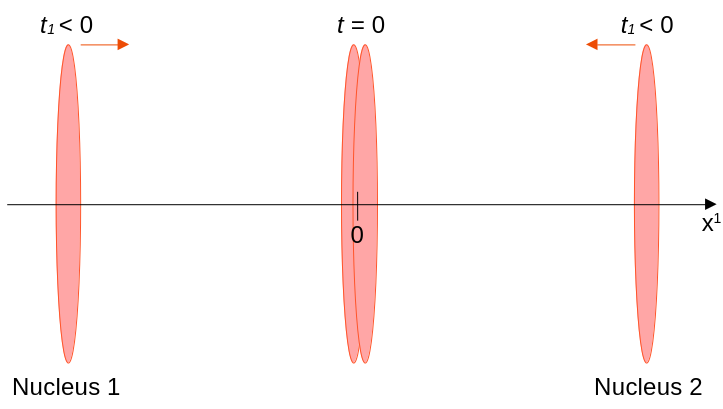
\includegraphics[width=0.7\textwidth]{Figures/HIC.png}
%    \caption{Two heavy nuclei, Lorentz-contracted into thin disks, travel along the $x^1$ axis in opposite directions until they collide at $t=0, x^1=0$.}
%    \label{fig:HIC}
%\end{figure}

\begin{figure}
	\centering
	\begin{tikzpicture}
	\filldraw[fill=red!20,draw=red!50] (-4,0) ellipse (0.2 and 1.5);
	\filldraw[fill=red!20,draw=red!50] (4,0) ellipse (0.2 and 1.5);
	\filldraw[fill=red!20,draw=red!50] (-0.1,0) ellipse (0.2 and 1.5);
	\filldraw[fill=red!20,draw=red!50] (0.1,0) ellipse (0.2 and 1.5);
	
	\node[above] at (-4,1.5) (t1) {$t_1<0$};
	\node[above] at (4,1.5) (t2) {$t_1<0$};
	\node[above] at (0,1.5) {$t=0$};	
	
	\node[below] at (-4,-1.5) {Nucleus 1};
	\node[below] at (4,-1.5) {Nucleus 2};
	
	\draw[-{Latex[length=2mm]},red]  (-3.8,1.5) -- ++(0.8,0);
	\draw[-{Latex[length=2mm]},red]  (3.8,1.5) -- ++(-0.8,0);
	
	\draw[-|] (-5,0) -- (0,0) node[at end, below] {$0$};
	\draw[-{Latex[length=3mm]}]  (0,0) -- (5,0) node[at end, below] {$x^1$};
\end{tikzpicture}
	\caption{Two heavy nuclei, Lorentz-contracted into thin disks, travel along the $x^1$ axis in opposite directions until they collide at $t=0, x^1=0$.}
	\label{fig:HI_CM_coll_axis}
\end{figure}

Prior to the collision, each nucleus's position four-vector, $x^\mu = (x^0,x^1,x^2,x^3) = (t,x,y,z)$, in Minkowski coordinates, is, in natural units ($c=\hbar=1$):
\begin{equation*}
\begin{split}
	\text{Nucleus 1}:& \quad (t,t,0,0) \\
	\text{Nucleus 2}:& \quad (t,-t,0,0)
\end{split}
\end{equation*}

These trajectories are well illustrated in the $x^1Ox^0$ plane (Fig. \ref{fig:HIC_lightcone}). 

%\begin{figure}
%    \centering
%    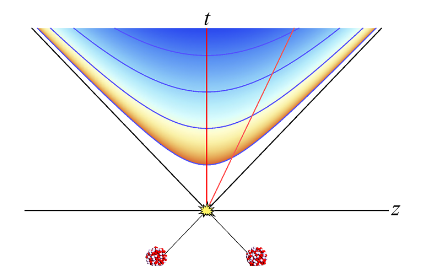
\includegraphics[width=0.7\textwidth]{Figures/HIC_lightcone.png}
%    \caption{A heavy-ion collision represented in the $x^1Ox^0$ %plane. Both nuclei travel along the light-cone centered around the collision at coordinates $(0,0)$. Taken from \cite{vanderschee2014}.}
%    \label{fig:HIC_lightcone}
%\end{figure}

\begin{figure}
    \centering
    %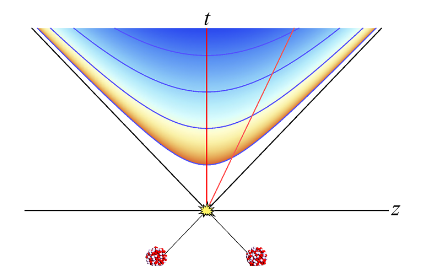
\includegraphics[width=0.7\textwidth]{Figures/HIC_lightcone.png} %PLACEHOLDER
    \begin{tikzpicture}[scale=1.5, every node/.style={transform shape=false}]
\begin{axis}[
	axis x line = center,
	axis y line = center,
	axis z line = none,
	%xlabel = $x^1$,
	%xlabel style={at={(axis description cs:1,0.1)}, anchor=north},
	%ylabel = $t$,
	%ylabel style={at={(axis description cs:0.44,1.05)}, anchor=west},
	%axis line style = {-},
	view={0}{90},
	xmin=-5,xmax=5,ymin=-0.5,ymax=5,
	unit vector ratio=1 1 1,	
	%x=1cm,y=1cm,
	xtick=\empty, ytick=\empty, ztick=\empty,
		]
\node at (0,0) (o) {};
    \addplot3 [
        surf,shader=interp,z buffer=sort,
        samples=60,
        domain=-3:3,
        y domain=1.25/1.414:5.2/1.414,
    ] (
{y*(exp(x)-exp(-x))/1.414},
{y*(exp(x)+exp(-x))/1.414},
{-(y-1/1.414)}
);
\draw[thick,samples=50,blue] plot (\x,{sqrt(1.56+\x*\x)});
\draw[thick,samples=50,blue] plot (\x,{sqrt(6.25+\x*\x)});
\draw[thick,samples=50,blue] plot (\x,{sqrt(13+\x*\x)});
\draw[thin,samples=51,black] plot (\x,{\x});
\draw[thin,samples=51,black] plot (\x,{-\x});

%\draw[-{Latex[length=2mm]},thick]  (o)+(-2.5,0) -- ++(2.5,0) node[below] {$x^1$};
%\draw[-{Latex[length=2mm]},thick]  (o)+(0,-0.2) -- ++(0,2.8) node[left] {$t$};
%\draw (o)+(-0.5,-0.5) -- ++(2.5,2.5);
%\draw (o)+(0.5,-0.5) -- ++(-2.5,2.5);

%\draw[draw opacity=0] (o) -- ++(2.5,2.5) node[pos=0.15,sloped,above,scale=0.6] {Pre-hydro};
\node at (0.1,0.35) [rotate=45,scale=0.5,right] {Pre-hydro};
\node [above=0.6 of o,scale=0.5,right] {QGP};
\node [above=1.7 of o,rotate=20,scale=0.5,right] {Hadronization};
\node [above=2.9 of o,rotate=15,scale=0.5,right] {Free Hadron Gas};

\node at (4.5,-0.3) [scale=0.66] {$x^1$};
\node at (-0.3,4.8) [scale=0.66] {$t$};

%\node [below left=0.6 of o] (n1) {};
%\node [below left=0.5cm of o] (m1) {};

%\node [below right=0.6 of o] (n2) {};
%\node [below right=0.5cm of o] (m2) {};


%\filldraw[fill=red!20,draw=red!50] (m1) ellipse (0.05 and 0.25);
%\filldraw[fill=red!20,draw=red!50] (m2) ellipse (0.05 and 0.25);
%\filldraw[fill=red!20,draw=red!50] (n1) ellipse (0.05 and 0.25);
%\filldraw[fill=red!20,draw=red!50] (n2) ellipse (0.05 and 0.25);

\end{axis}
\end{tikzpicture}
    \caption{A heavy-ion collision represented in the $x^1Ox^0$ plane. Both nuclei travel along the light-cone centered around the collision at coordinates $(0,0)$. The several stages of the post-collision inter-nuclear medium are delimited (not to scale). Based on the figure from \cite{vanderschee2014}.}
    \label{fig:HIC_lightcone}
\end{figure}

After the collision, many of the nuclei's constituent particles
carry on in the direction they were moving at the speed of light, and the pre-hydrodynamic medium which will be studied in this work forms in between the now receding discs.
%After the collision, the nuclei's approximately static high-$x$ partons, discussed in Section \ref{sec:scale_separation}, carry on in the direction they were moving at the speed of light, acting as color sources for the gluon fields then generated in the space between the now receding nuclei.
%\textcolor{red}{[They were already acting as color sources for fields, but in the other quadrants]}.
Fig. \ref{fig:HIC_lightcone} suggests the usefulness of a coordinate system where the axes lie along the nuclei's path in the $x^1Ox^0$ plane. In the Light-Cone coordinate system (see Appendix \ref{ap:Light_Cone}), 
\begin{subequations}
\begin{gather}
x^+ = \frac{x^0+x^1}{\sqrt{2}} \\
x^- = \frac{x^0-x^1}{\sqrt{2}}
\end{gather}
\end{subequations}
In this coordinate system, the nuclei's position four-vectors, $x^\mu=(x^+,x^-,x^2,x^3)$, are:
\begin{equation*}
\begin{split}
	\text{Nucleus 1}:& \quad (\sqrt{2}t,0,0,0) \\
	\text{Nucleus 2}:& \quad (0,\sqrt{2}t,0,0)
\end{split}
\end{equation*}
and the collision coordinates remain at $(x^+=0,x^-=0)$.

Having presented its natural coordinate system, the effective theory within which this work was produced may be introduced.

%\textcolor{purple}{In order to fulfill this work's objectives, it will be necessary to calculate the gluon fields generated in the space between the receding nuclei, making use of the classical Yang-Mills equations. The fields will be determined from the the static distributions of color charge of the receding nuclei.}

%\textcolor{red}{Move the introduction to dEdx and $\hat{q}$ to before this? say they are the result of the color fields acting on the quark probe?}


\section{The Color Glass Condensate and The McLerran-Venugopalan Model}
%\textcolor{purple}{Should I start with describing protons with the CGC and say it's the same for the nuclei? or should I start right away using the word nucleus?}

%\textcolor{blue}{[Separation between the CGC and the MV model]}

The \gls{CGC} is an effective theory of \gls{QCD} for high-energy %\gls{QCD} 
scattering applied to describe the aforementioned saturated gluons \cite{Gelis_2010}, which evade standard perturbation techniques. It is one of the approaches adopted to study initial state effects in \glspl{HIC}; that is, the properties of the system prior to the formation of the \gls{QGP}, and their impact on final-state observables. It is used, for example, in the modeling of the incoming nuclei and of the non-equilibrated medium that leads to the \gls{QGP}, which in this context earns the name ``glasma''.  In this regard, it has stood out due to its practical applicability and phenomenological success. \cite{Albacete_2014} 

The effective theory hinges on the partition of the parton content of a hadron,
%-- in this case, a heavy nucleus --
 through approximations, into static color charges and the saturated gluons (represented by dynamic classical gluon fields) which they generate via the processes described in Section \ref{sec:gluon_saturation}. \cite{Gelis_2010} In this case, the hadron in question is a heavy nucleus, which is made up of neutrons and protons whose contents were previously discussed. This partition is done in the \gls{IMF}, where the nucleus is boosted along its direction of motion in order to make all of its constituents' momenta approximately collinear to its own.
\glsreset{IMF}
%The \gls{CGC} effective theory of \gls{QCD} for high-energy \gls{QCD} scattering is one of the approaches used to study initial state effects in \glspl{HIC}, and has stood out due to its practical applicability and phenomenological success. \cite{Albacete_2014}

%\textcolor{purple}{- Separation of the contents of the nucleus//hadron according to their momentum. This is done in the INFINITE MOMENTUM FRAME.}

The founding, classical iteration of this formalism was introduced in \cite{McLerran_1994_classic_source} and is known today as the \gls{MV} model. Presently, the \gls{CGC} corpus includes quantum corrections to the \gls{MV} model, and effective theories that take other models as a starting point.

%Together with other iterations, which incorporate quantum corrections to the classical theory, they form the corpus of the \gls{CGC} framework.

\subsection{Classical saturated gluon fields}
%\textcolor{purple}{YET UNJUSTIFIED: why $N \sim 1/g^2$; why $g$ is small; well sourced?}

First, the treatment of the saturated gluons as classical fields will be justified. Reaching the saturation regime implies that the non-linear terms of the evolution equation have become non-negligible\footnote{Here, specifically, the \gls{BK} equation at leading order is considered, where it serves as a non-linear extension of the \gls{BFKL} evolution equation. \cite{Albacete_2014}}, as discussed in Section \ref{sec:gluon_saturation}. For this to occur, gluon densities should be of the order $\sim 1/\alpha \sim 1/g^2$. When taking the gluon density as a proxy for the gluon field two-point function, $\left< AA \right>$, this allows estimating the average value of the gluon fields as $\sim 1/g$
%The saturated gluon densities at low-$x$ discussed previously in Sections \ref{sec:nuclear_matter} and \ref{sec:gluon_saturation} imply gluon fields of the order $A \sim 1/g$
, which does not allow their treatment through standard perturbative techniques\footnote{For example, in calculating the matrix element $\mathcal{M}$ for a \gls{QCD} process using a series expansion in powers of $g$, all terms are proportional to $gA \sim \mathcal{O}(1)$, which does not allow truncating the series in order to estimate $\mathcal{M}$ -- all orders need to be summed.}. \cite{Albacete_2014} However, it opens the possibility of their treatment as classical fields.

Comparing the occupation number of the saturated gluon fields, which is itself a proxy for the gluon field two-point function, and the commutator of their creation and annihilation operators, $a$ and $a^\dagger$, \citep{Albacete_2014} in the regime of perturbative \gls{QCD},
\begin{equation}
	N = a^\dagger a \sim \frac{1}{g^2} \quad \gg \quad [a^\dagger, a] \sim 1
\end{equation}
it is possible to state that quantum corrections to the classical solution, where the fields commute, are negligible. Thus, it is reasonable to treat the low-$x$ gluon fields as classical fields. This is the basis for the development of the \gls{MV} model.

\subsection{Partition of the nucleus's parton content} \label{sec:scale_separation}

In order to analytically validate the partition of the parton content of the nucleus into a static and a dynamic part in a \gls{HIC}, it is necessary to move to the \gls{IMF}. In the \gls{IMF}, the nucleus is boosted along its direction of motion so as to make the momenta of its constituent partons approximately collinear to its own. In this frame, considering a nucleus moving in the positive $x^1$ direction with large total longitudinal momentum $P$ much greater than its mass, $m_A$, the four-momenta of the nucleus and of one of its constituent partons in Minkowski coordinates are: \cite{Thomson8:2013}
\begin{subequations}
\label{eq:IMF}
\begin{align}
	\text{Nucleus: } & P^\mu = (P,P,0,0)
	&
	\text{Parton $i$: } & p^\mu = (x_i P, x_i P, \sim 0, \sim 0)
\\
\intertext{
where $0<x_i<1$ is the fraction of the nuclear longitudinal momentum carried by the $i$-th parton; it was further assumed that the boost applied was such that $x_i P \gg m_i$, with $m_i$ being the $i$-th parton's mass. In light-cone coordinates,}
	\text{Nucleus: } & P^\mu = (P^+,0,0,0)
	&
    \text{Parton $i$: } & p^\mu = (x_i P^+, \sim 0, \sim 0, \sim 0)
\end{align}
\end{subequations}
where $P^+ = \sqrt{2} P$. It becomes clear that $x_i$ is also the $i$-th parton's fraction of the nuclear light-cone $+$-momentum.

%\textcolor{red}{- Problem: not all of the boosted partons will obey $p_i^2 \gg m_i^2$ right? or even $p^1 \gg p_T$}

The uncertainty principle can be used to estimate the approximate extent of each parton over the $x^-$ and $x^+$ coordinates: \cite{Lappi_notes,Albacete_2014}
\begin{subequations} \label{eq:Uncertainty_Relations}
\begin{gather}
\Delta x^- \propto \frac{1}{p^+} = \frac{1}{x_i P^+} \\
\Delta x^+ \propto \frac{1}{p^-} = \frac{2p^+}{(p^0)^2 - (p^1)^2} = \frac{2p^+}{(\mathbf{p}_\perp)^2 + {m_i}^2} \approx \frac{2 x_i P^+}{(\mathbf{p}_\perp)^2}
\end{gather}
\end{subequations}
where $\mathbf{p}_\perp$ is the $i$-th parton's transverse momentum, which was taken to be negligible in Eqs. (\ref{eq:IMF}) when compared to its longitudinal momentum.

Two useful conclusions about the $x^+,x^-$  scales of high-$x$ and low-$x$ partons may be extracted from the uncertainty relations:
\begin{itemize}
	\item[1)] high-$x$ partons are highly localized in the $x^-$ direction. That is, they occupy a very thin ``slice" of space in the $x^-$ direction.
	\item[2)] high-$x$ partons are more delocalized in the $x^+$ direction than their low-$x$ counterparts. That is, their typical $x^+$ scale %\textcolor{red}{(often called light-cone time -- introduce $x^+/t$ equivalence somewhere??)}
is greater than the low-$x$ partons'. Equivalently, the fluctuations of the low-$x$ parton fields are much shorter along the $x^+$ direction than for the high-$x$ parton fields.
\end{itemize}

%\textcolor{purple}{? Include the naive \cite{Lappi_notes} interpretations? 1) the Lorentz-contraction of the nucleus along $x^1$. 2) Time dilation experienced by valence partons.}

It is from the second point that a hierarchy arises, central to the \gls{CGC} formalism, of partons separated according to their $x$-values. A $+$-momentum scale, $\Lambda^+$, is introduced to separate the high-$x$, or valence, partons and the low-$x$ partons. From the perspective of the low-$x$ partons, the valence partons have very slow dynamics
%\textcolor{red}{ \footnote{\textcolor{blue}{Also slow in the timescale of the pre-hydrodynamic stage?}}}
in $x^+$. In the limit of this argument, they are \emph{static} in $x^+$; for particles traveling at the speed of light, being static in $x^+$ is equivalent to being static in $t$. As such, in the \gls{CGC}, valence partons become constant color charges, which serve as sources for the \emph{dynamic} low-$x$ parton fields.
% Regarding the low-$x$ partons,
As was introduced in sections \ref{sec:nuclear_matter} and \ref{sec:gluon_saturation}, the partonic content of protons, and hence of the nucleus, is dominated by gluons at low-$x$. Therefore, the dynamic fields are taken to be purely gluon fields.

%Regarding the low-$x$ partons, they are, in contrast, dynamic. Additionally since the partonic content of protons, \textcolor{blue}{ and hence of the nucleus}, is dominated by gluons at low-$x$, as introduced in sections \ref{sec:nuclear_matter} and \ref{sec:gluon_saturation}, these dynamic fields are taken to be gluonic fields, also called color fields.

%The parton content of the nucleus is thus divided into the group of high $+$-momentum ($p^+ > \Lambda^+$) static color charges and the group of low $+$-momentum ($p^+ < \Lambda^+$) dynamic classical gluon fields which they generate. The static color charges may themselves be treated as classical \citep{Albacete_2014,McLerran_1994_classic_source} and are eikonally \textcolor{red}{define} coupled to the classical gluon fields; that is, they suffer negligible recoil from their interactions with the color fields, when compared to their longitudinal momentum.\cite{Gelis_2010} Thus, they are introduced into the \gls{QCD} Lagrangian (Eq. (\ref{eq:QCD_Lagrangian_Indices})) as a classical color current 4-vector, $J^\mu \equiv J^\mu_a T^a$, in the term $A_\mu^a J^\mu_a$. Since, now, the formalism does not include quantum quark fields, Eq.  (\ref{eq:QCD_Lagrangian_Indices}) becomes 

The parton content of the nucleus is thus divided into the group of high $+$-momentum ($p^+ > \Lambda^+$) static color charges and the group of low $+$-momentum ($p^+ < \Lambda^+$) dynamic classical gluon fields which they generate. The static color charges may themselves be treated as classical \citep{Albacete_2014,McLerran_1994_classic_source}, and are expressed in the formalism as a classical color current four-vector, $J^\mu \equiv J^\mu_a T^a$. This current is eikonally coupled to the classical gluon fields; that is, the static charges of the current suffer negligible recoil from their interactions with the gluon fields, when compared to their longitudinal momentum. \cite{Gelis_2010} This coupling is expressed by inserting the color current into the Lagrangian via the term $A_\mu^a J^\mu_a$. Since, now, the formalism does not include quantum quark fields, Eq.  (\ref{eq:QCD_Lagrangian_Indices}) becomes 

%\textcolor{red}{the absence of dynamic color fields gets rid of the first term. The influence of the static color sources on the system is brought back via the} addition of an external color source term to the \gls{QCD} Lagrangian. Equations \ref{eq:QCD_Lagrangian} and \ref{eq:QCD_Lagrangian_Indices} become, respectively,
\begin{equation}
	\mathcal{L}_\text{QCD}'  =  - \frac{1}{4} F_{\mu \nu}^a F^{\mu \nu}_a + A_\mu^a J^\mu_a 
	\label{eq:QCD_Lag_Current_indices}
\end{equation}
where $J^\mu \equiv J^\mu_a T^a$. The Lagrangian is thus written in terms of a static color current $J$, representing the high-$x$ partons, and of dynamic gluon fields $A$, representing the low-$x$ gluons.

Consequently, the corresponding Euler-Lagrange equations for the gluon fields $A^\mu$ become:
\begin{equation}
	[D_\mu, F^{\mu \nu}] = J^\nu
\end{equation}
which, provided an expression for the external color current, may be solved for the classical gluon fields.

Seeing as $J^\mu$ describes partons traveling at near the speed of light in the $x^1$ direction, then, in light-cone coordinates, its only non-vanishing component is $J^+$ . Additionally, it will directly depend on the number color charge distribution of the valence partons, $\rho (x^\mu) \equiv \rho_a(x^\mu) T^a$.
%\begin{gather}
%	J^\mu = \delta^\mu_+ J^+ \label{eq:Nonvanishing_current_+} \\
%	J^+(x^\mu) = g \rho (x^\mu) \label{eq:J_from_rho}
%\end{gather}
From the previous discussion on the static nature of the color charges, $\rho$'s dependence on $x^+$ can be dropped. Furthermore, due to the first conclusion drawn from the uncertainty relations (Eqs. \ref{eq:Uncertainty_Relations}), the color charge distribution function of the static valence partons should be very thin in the $x^-$ direction. 
%In the limit where this thin $x^-$ dependence factorizes to a Dirac-delta function, 
The valence color current becomes, in light-cone coordinates:
\begin{equation}
	{J}^\mu (x^-,\mathbf{x}_\perp) = (g \rho (x^-,\mathbf{x}_\perp), \sim 0, \sim 0, \sim 0)
	\label{eq:+_Current}
\end{equation}
where the charge distribution is taken to be very narrowly peaked around $x^-=0$.
%$\rho$ has become an area number charge density \textcolor{purple}{(why?)}.

\subsection{The stochastic nature of $\rho$}
The color charge distribution $\rho$, from which $J^\mu$ and, consequently, the evolution of the gluon fields are obtained, is fixed for a single nucleus in a single event. It is different, however, for different nuclei and for each event. For this reason, it is treated as a stochastic variable \cite{Gelis_2010} which is neither accessible experimentally for each collision nor computable from first principles.  Even considering a single nucleus, $\rho$ would change if enough time is allowed to pass in order for the nucleus to travel over a $x^+$ length greater than the valence partons' typical $x^+$ scale \cite{Gelis_Habilitation}. In order to calculate an observable $\mathcal{O}$ out of many events within the \gls{CGC} effective theory, one must determine its average value considering all the different possible color charge distributions and their probabilities: \cite{Gelis_2010}
\begin{equation}
	\left< \mathcal{O} \right> = \int [\diff \rho] W[\rho] \mathcal{O}[\rho]
\end{equation}
where $\mathcal{O}[\rho]$ is the observable's value for the particular charge distribution $\rho$, and $W[\rho]$ is a functional probability distribution evaluated for that same charge distribution.%, describing its probability of occurring.

\subsection{Quantum Corrections and the McLerran-Venugopalan Model}

So far, the framework's dependence on the arbitrary choice of a $+$-momentum scale $\Lambda^+$ which separates low- and high-$x$ partons has been neglected. Indeed, once a $+$-momentum scale has been set, one neglects that certain low-$x$ partons sorted into the category of classical fields may actually act as static color sources for lower-$x$-still partons\footnote{In the language of Section \ref{sec:gluon_saturation}, even a low-$x$ gluon can serve as an emitter of lower-$x$ gluons.} \cite{Albacete_2014}. 
Thus, choosing a different $\Lambda^+$ leads to different final-state observable values, amounting to a quantum correction to the classical theory.
%Consider changing the momentum scale from an initial value of $\Lambda_+$ to $\Lambda'_+$ -- this alters the value of final-state observables calculated with the \gls{CGC} framework. 
%In order to incorporate these quantum corrections into the effective theory,
However, $W$, $\rho$ or correlators of $\rho$ may be renormalized, so as to incorporate the effect of these low-$x$ emmiters into the theory by changing the distribution of static sources. 
%However, it is possible to renormalize $\rho$, correlators of $\rho$ or the probability distribution $W$ so as to incorporate these quantum corrections into the \gls{CGC} effective theory. This preserves the value of the observables, making them independent of $\Lambda^+$ while keeping the calculation procedure strictly classical \citep{Albacete_2014}.  
This keeps the calculation strictly classical while incorporating quantum corrections. \citep{Albacete_2014}
Choosing to incorporate the quantum corrections into $W$, which then becomes dependent on the $+$-momentum scale, $W_{\Lambda^+}$, its evolution with $\Lambda^+$ is ruled by the \gls{JIMWLK} equation (read ``Jim-Walk") \cite{Gelis_2010}.
%Other methods to incorporate quantum corrections into the effective theory exist, as well as variations on the \gls{JIMWLK} equation \citep{Albacete_2014}.

In spite of this achievement, an initial probability distribution $W_{\Lambda^+_0}$ is still necessary before studying its evolution with the $+$-momentum scale $\Lambda^+$; this function can be seen as an initial condition for the \gls{JIMWLK} equation. The \gls{MV} model, the founding iteration of the \gls{CGC}, provides that initial condition, $W_{\text{MV}}$, for the case of large nuclei.

The \gls{MV} model's functional probability distribution $W_{\text{MV}}$ %and corresponding charge density 2-point correlator are 
is motivated physically by the characteristics of large nuclei: \citep{Gelis_Habilitation}
\begin{itemize}
	\item[1)] Due to color confinement, color charge within different nucleons should be uncorrelated. Since charge densities at different transverse positions $\mathbf{x}_\perp$ and $\mathbf{y}_\perp$ are associated with different nucleons/longitudinal superpositions of nucleons, $\rho(\mathbf{x}_\perp)$ and $\rho(\mathbf{y}_\perp)$ should also be uncorrelated.
	\item[2)] For large nuclei, at least at central positions, transverse color charge density results from the sum of many longitudinally aligned nucleons. Since the color charge of those nucleons is uncorrelated, then $\rho(\mathbf{x}_\perp)$ is a sum of uncorrelated variables. Therefore, the Central Limit Theorem applies, and $\rho(\mathbf{x}_\perp)$ should follow a Gaussian distribution.
\end{itemize}

The form of $W_{\text{MV}}$, apart from a normalization constant $C$, is \citep{Albacete_2014} \textcolor{red}{\citep{Carrington_2022}}:

%\textcolor{blue}{[Some authors use $\mu(x^-)$, $\rho(x^-, \mathbf{x}_\perp)$ for $W$ \citep{Albacete_2014} or for the 2-point correlator \cite{Lappi_notes}. From what I saw, only \cite{Gelis_Habilitation} introduces the MV model without the $x^-$ coordinate here, but for $W[\rho_a]$ instead of $W[\rho]$.][Should I not factorize the $x^-$ as soon as I do, so that I can use those results here?]}
\begin{equation}
	W_\text{MV}[\rho] = C \exp \left[ - \int \diff x^- \diff^2 \mathbf{x}_\perp \frac{\rho^a(x^-,\mathbf{x_\perp})\rho^a(x^-,\mathbf{x_\perp})}{2 \mu(x^-)^2 } \right]
\end{equation}
which has an associated charge density two-point correlator:
\begin{equation}
	\left< \rho_a(x^-,\mathbf{x}_\perp) \rho_b (y^-,\mathbf{y}_\perp) \right> =  \delta^{ab} \delta^2 (\mathbf{x}_\perp - \mathbf{y}_\perp) \delta (x^- - y^-) \mu_A^2 \lambda(x^-, \mathbf{x}_\perp)
	\label{eq:MV_charge_correlator}
\end{equation}
%\textcolor{red}{How do I relate these two?}

%\textcolor{red}{[Explain $\mu/\lambda$].}

In spite of not incorporating quantum corrections, the \gls{MV} model may be used directly, without needing to be evolved into $x$-scales much smaller than $\Lambda_0^+$, for the study of $pA$ or $AA$ collisions where the values of $x$ are not small enough to require that evolution. \citep{Gelis_2010} 

%that constitute the classical color fields and the color charge sources

%\textcolor{blue}{[Talk about renormalization of the theory and the JIMWLK equations?] }

%\textcolor{red}{When to make the leap from the particle description of the mechanisms of parton creation/annihilation into classical fields.}

%- Description of the two classes of partons. Justified on Heisenberg uncertainty principle, delocalization in x- and x+ coordinates. Explain why only gluons in the lower class.

%Combining the separation of partons into static color charges and dynamic gluon fields with the classical treatment of those fields, \textcolor{red}{it is possible to study the system by solving the classical Yang-Mills equations (Eq. \ref{eq:Yang-Mills}) using Eq. \ref{eq:+_Current} as the external color current.}



%\textcolor{blue}{[Explanation of the classical low-$x$ gluon fields.]}


%\textcolor{purple}{The \gls{MV} model -- MODEL OF WHAT. INTRODUCED IN ... BY ... .}


%\textcolor{purple}{- Then the stochastic, Gaussian model for the static color charges (fuzzy)}

The classical \gls{MV} model will be used, and quantum corrections will be left out of the scope of this work. The application of this formalism to the two-nuclei system of a \gls{HIC} will be introduced over the next sections. 



\section{Solving the Yang-Mills Equations}
\label{sec:solving_YM}

\subsection{One nucleus}
First, the case of a single nucleus will be considered.  Nucleus 1 is chosen, moving in the positive $x^1$ direction.
Solutions to the Yang-Mills equations for a single nucleus moving along the light-cone were first found analytically in \cite{McLerran:1993ka} for the classical case $D_{\mu}F^{\mu \nu} = J^\nu$.   %\textcolor{blue}{The very first papers' approach was to start off in light-cone gauge right away. Should I refer to this method too?}

In the present work, the Yang-Mills equations in the case of a single nucleus are initially solved in the Lorenz, or covariant, gauge, where $\partial_\mu A^\mu=0$, following %the more recent solving of the full equations from 
%\cite[Section 2.2]{Blaizot_2004}
\cite{Blaizot_2004}\footnote{Note that this paper's covariant derivative definition is $D_\mu=\partial_\mu -igA_\mu$. However, this does not affect the final result.}. The solution is then brought to light-cone gauge, where $A^+=0$, an axial gauge condition, following the approach from 
%\citep[Section 3A]{Carrington_2022}.
\citep{Carrington_2022}. 
%\textcolor{blue}{(\citep{Kovner_1995}: "Using light cone gauge one has direct access to the gluon distribution functions of the parton model" -- I wasn't able to find a justification for this, in order to include it as a motivation to work in light-cone gauge. Is there any reference you know I could use?)}.
Bringing the final solution to light-cone gauge is necessary, as this is the gauge where the parton distribution operators have the physical interpretation of quantifying the parton populations inside a hadron.
% \citep{Kovner_1995}\citep[Section 5.1.1]{Lappi_high_energy}\citep[Section 2.4]{Iancu:2000hn}
\citep{Kovner_1995,Lappi_high_energy,Iancu:2000hn} Thus, this gauge is required in order to use our previous insights concerning the low-$x$ gluon populations within protons. Additionally, use of the light-cone gauge allows reducing the problem to two degrees of freedom, the transverse components of $A^\mu$. 
%\citep[Section 5.1.1]{Lappi_high_energy}
\citep{Lappi_high_energy}

First of all, the equation explicitly enforcing the covariant conservation of color charge is added to the set of equations to solve. It is analogous to Classical Electrodynamics' equation of conservation of electric charge, and is obtained from the Yang-Mills equations as:
\begin{equation}
	[D_\mu, F^{\mu \nu}] = J^\nu \implies [D_\nu, J^\nu] = [D_\nu, [D_\mu, F^{\mu \nu}]] = 0
	\label{eq:covariant_conservation}
\end{equation}
via the Jacobi identity and the $F^{\mu \nu} = -ig [D_\mu, D_\nu]$ identity for the gluon field strength tensor (see Appendix \ref{ap:covariant_conservation} for a detailed derivation). %\textcolor{red}{Expanding for a four-current with only a $+$-component:
%\begin{equation}
	%\partial_+ J^+ = ig[A_+,J^+] = ig[A^-,J^+]
%\end{equation}
%$J^+$ is required to evolve in light-cone time ($x^+$) provided that the left side does not vanish. The right side vanishes for the assumed form of the current (Eq. (\ref{eq:+_Current})), however the solution for $A^\mu$ that will be produced in this section, out of a current of the form of Eq. (\ref{eq:+_Current}), will guarantee that the left side vanishes as well.}

The conservation equation and the Yang-Mills equations (in the Lorenz gauge) are then arranged into the system of equations:
\begin{equation}
	\begin{cases}
	[D_\mu, J^\mu] = 0 \\
	[D_\mu, F^{\mu \nu}] = J^\nu
	\end{cases} \Leftrightarrow
	\begin{cases}
	\partial_\mu J^\mu = -ig[A_\mu, J^\mu]  \\
	\partial_\mu \partial^\mu A^\nu = J^\nu - ig [A_\mu, F^{\mu \nu} + \partial^\mu A^\nu]
	\end{cases}
\end{equation}

A solution may be built by solving this system iteratively, for the fields and current expanded in terms of powers of the color number charge density, $\rho$. The terms of order $(n)$ are obtained from those of lower orders by:
\begin{equation}
	\begin{cases}
	\partial_\mu J_{(n)}^\mu = -ig[A_\mu, J^\mu]_{(n)}  \\
	\partial_\mu \partial^\mu A_{(n)}^\nu = J_{(n)}^\nu - ig [A_\mu, F^{\mu \nu} + \partial^\mu A^\nu]_{(n)}
	\end{cases}
\end{equation}

%\begin{equation}
%	\begin{cases}
%	\partial_\mu J_{(n+1)}^\mu = ig[A^{(n)}_\mu, J_{(n)}^\mu]  \\
%	\partial_\mu \partial^\mu A_{(n+1)}^\nu = J_{(n+1)}^\nu + ig [A^{(n)}_\mu, F_{(n)}^{\mu \nu} + \partial^\mu A_{(n)}^\nu]
%	\end{cases}
%\end{equation}

Inputting $J_{(0)}^\mu = A_{(0)}^\mu = 0$ (since, in the absence of color charges, there are neither any color currents nor fields generated from them) and $J_{(1)}^\mu = g \delta^{\mu}_+ \rho(x^-,\mathbf{x}_\perp)$  (Eq. (\ref{eq:+_Current})), the top equation for $n=1$ is automatically satisfied since $\partial_+ J^+_{(1)} = 0$. The bottom equation may be solved by requiring that $A^\mu_{(1)}$, like $J_{(1)}^\mu$, be independent of $x^+$, and that it vanishes in the far past \citep{Blaizot_2004}: 
%\textcolor{blue}{(does not explode in the far past? But this is a transverce laplacian; it would explode away from the nucleus)}
\begin{equation}
\begin{split}
	\partial_\mu & \partial^\mu A_{(1)}^\nu = J_{(1)}^\nu ~ \to ~
	 - \mathbf{\nabla}_\perp^2 A_{(1)}^\nu = J_{(1)}^\nu \\
	 & \to ~ A^\nu_{(1)}(x^-,\mathbf{x}_\perp) =  g \delta^{\nu}_+  \int \diff^2 \mathbf{y}_\perp \mathcal{G}(\mathbf{x_\perp} - \mathbf{y_\perp}) \rho(x^-,\mathbf{y}_\perp)
\end{split}
\label{eq:n_1_A}
\end{equation}
where $\mathcal{G}(\mathbf{x_\perp} - \mathbf{y_\perp})$ is a Green's function for the 2-dimensional Laplacian, $-\mathbf{\nabla}_\perp^2 = \partial_i \partial^i$ with $i=2,3$.

Moving to the $n=2$ system, the right side of the top equation is once again $0$ since $A_{(1)}^\mu$ and $J_{(1)}^{\mu}$ only have a $+$-component. For the bottom equation, its commutator vanishes because $A_{(1)}^\mu$ only has a $+$-component and because that component is independent of $x^+$. The system for $n=2$ is, then,
\begin{equation}
	\begin{cases}
	\partial_\mu J_{(2)}^\mu = 0  \\
	\partial_\mu \partial^\mu A_{(2)}^\nu = J_{(2)}^\nu
	\end{cases}
\end{equation}

Once again requiring that the current and fields vanish in the far past
%do not explode in the far past
, the solution is $J_{(2)}^\mu = 0$ for the top and $A_{(2)}^\mu =0$ for the bottom. This makes all the greater-order terms also $0$, making the final solution equal to the first order solution:
\begin{subequations}
\begin{gather}
	J^\mu(x^-,\mathbf{x}_\perp) = g \delta^{\mu}_+ \rho(x^-,\mathbf{x}_\perp) \\
	A^\nu(x^-,\mathbf{x}_\perp) =  g \delta^{\nu}_+  \int \diff^2 \mathbf{y}_\perp \mathcal{G}(\mathbf{x_\perp} - \mathbf{y_\perp}) \rho(x^-,\mathbf{y}_\perp)
\end{gather}
\end{subequations}

Finally, in order to move to light-cone gauge, where the $+$-component of $A$ is null, the appropriate gauge transformation matrix $U$ must be found:
\begin{equation}
	A^\mu_\text{LC} = U^\dagger A^\mu U + \frac{i}{g} U^\dagger \partial^\mu U
\label{eq:gauge_transformation}
\end{equation}

It may be found by solving the equation:
\begin{equation}
	A_{\text{LC}}^{+}=0 ~ \Leftrightarrow ~ U^\dagger A^+ U + \frac{i}{g} U^\dagger \partial^+ U = 0 ~ \Leftrightarrow ~ A^+ U + \frac{i}{g} \partial_- U = 0 ~ \Leftrightarrow ~ \partial_- U = ig A^+ U
\end{equation}
which admits a solution of the type $U(x^-,\mathbf{x}_\perp)$ and may be solved iteratively in its integral form:
\begin{gather}
	U(x^-,\mathbf{x}_\perp) = U(x^-_0, \mathbf{x}_\perp) + ig \int_{x^-_0}^{x^-} \diff z A^+ (z, \mathbf{x}_\perp) U (z, \mathbf{x}_\perp)
\end{gather}
\begin{alignat}{2}
	U(x^-,\mathbf{x}_\perp) & = \lim_{n \to \infty} \Bigg( \mathds{1} 
	 && + ig\int_{x_0^-}^{x^-}  \diff z_0 A^+ (z_0) 
	+ (ig)^2\int_{x_0^-}^{x^-} \diff z_0 \int_{x_0^-}^{z_0} \diff z_1 A^+ (z_0) A^+ (z_1) + ... \nonumber \\ 
	& && + (ig)^n\int_{x_0^-}^{x^-} \diff z_0  \int_{x_0^-}^{z_0} \diff z_1 ...  \int_{x_0^-}^{z_{n-1}} \diff z_n ~ A^+ (z_0) A^+ (z_1) ...  A^+ (z_n)
	 \Bigg) U(x_0^-,\mathbf{x}_\perp) \nonumber \\
	 & = \lim_{n \to \infty} \Bigg( \mathds{1} 
	 && + ig\int_{x_0^-}^{x^-}  \diff z_0 A^+ (z_0) 
	+ \frac{(ig)^2}{2} \int_{x_0^-}^{x^-} \diff z_0 \int_{x_0^-}^{x^-} \diff z_1  \mathcal{P}^- \Big \{ A^+ (z_0) A^+ (z_1) \Big \} + ... \nonumber \\ 
	& && + \frac{(ig)^n}{n!}\int_{x_0^-}^{x^-} \diff z_0  \int_{x_0^-}^{x^-} \diff z_1 ...  \int_{x_0^-}^{x^-} \diff z_n ~ \mathcal{P}^- \Big \{ A^+ (z_0) A^+ (z_1) ...  A^+ (z_n) \Big \}
	 \Bigg) U(x_0^-,\mathbf{x}_\perp) \nonumber \\
	 & \equiv \mathcal{P}^- \exp  \Bigg[&& ig \int_{x^-_0}^{x^-} \diff z A^+ (z, \mathbf{x}_\perp) \Bigg] U(x_0^-,\mathbf{x}_\perp)
\end{alignat}
where the dependence of the $A^+$ fields on $\mathbf{x}_\perp$ was only shown explicitly in the last line and $\mathcal{P}^-$ is the path-ordering operator for the $x^-$ variable; that is, it orders the $A^+$ field operators from right to left in descending order of their $x^-$ argument:
\begin{gather}
	x^-_n \geq x^-_{n-1} \geq ... \geq x_1^- \implies \mathcal{P}^- \left \{A^+(x^-_{p_n}) A^+(x^-_{p_{n-1}}) ... A^+(x_{p_1}^-) \right \} \equiv A^+(x^-_n) A^+(x^-_{n-1}) ... A^+(x_1^-) \\
	\text{with $\{p_n, p_{n-1}, ..., p_1\}$ some permutation of $\{n, n-1, ..., 1\}$} \nonumber
\end{gather}
Additionally,  $\mathcal{P}^-\exp[ig\int_{x^-_0}^{x^-} \diff z A^+ (z, \mathbf{x}_\perp)]$ is called the path-ordered exponential of the $ig\int_{x^-_0}^{x^-} \diff z A^+ (z, \mathbf{x}_\perp)$ integral.

This solution corresponds to a Wilson Line,
\begin{equation}
	\mathcal{P}^- \exp  \Bigg[ig \int_{x_0^-}^{x^-} \diff z A^+ (z, \mathbf{x}_\perp) \Bigg] \equiv W[A^+](x^-, x_0^-,\mathbf{x}_\perp)
\end{equation}
These objects frequently appear in calculations in the \gls{CGC} framework. One physical interpretation of a Wilson Line is as the matrix for the rotation in color space that a high-energy quark experiences when traversing a color field eikonally -- that is, having negligible momentum exchange with the color field \cite{Solana_lectures}. Indeed, one way to turn the initial expression for the color current (Eq. (\ref{eq:+_Current})) into a covariantly conserved one is to add Wilson line operators to it reflecting the color rotation it suffers as it traverses the gluon fields: $J^\mu(x^-,\mathbf{x_\perp}) \to W[A^-](x^+,x^+_0,\mathbf{x_\perp}) J^\mu(x^-,\mathbf{x_\perp}) W[A^-](x^+_0,x^+,\mathbf{x_\perp})$. Here, the Wilson lines serve as link operators bringing the original (at $x_0^+$) current, $J^\mu$, to the present, $x^+$. 

It is possible to choose $x^-_0$ to be $-\infty$ and $U(x_0^-,\mathbf{x}_\perp)$ to be $\mathds{1}$ with $U$ remaining a solution: %\textcolor{red}{(Is this a part of residual gauge freedom?}
\begin{equation}
	U(x^-,\mathbf{x}_\perp) = \mathcal{P}^- \exp  \Bigg[ig \int_{-\infty}^{x^-} \diff z A^+ (z, \mathbf{x}_\perp) \Bigg]
\end{equation}
 %\textcolor{purple}{(Should add some reference to the celebrity of Wilson Lines in ths line of work.)}

Renaming the $+$-component of $A$ in the Lorenz gauge to $\Phi(x^-,\mathbf{x}_\perp)$,
% and dropping the ``LC" subscript to denote fields in the light-cone gauge, 
the expressions for the gluon fields in light-cone gauge become:
\begin{subequations}
\begin{alignat}{2}
	A^+_\text{LC} & = 0 && \\
	A^-_\text{LC} & = 0 && \\
	A^i_\text{LC} & = \frac{i}{g} U(x^-,\mathbf{x}_\perp)^\dagger ~ && \partial^i U(x^-,\mathbf{x}_\perp), \qquad i = 2,3\\
	& \text{with} ~ U(x^-, \mathbf{x}_\perp) && =
	\mathcal{P}^- \exp  \Bigg[ig \int_{-\infty}^{x^-} \diff z ~ \Phi (z, \mathbf{x}_\perp) \Bigg] \nonumber \\ 
	&  &&  =  \mathcal{P}^- \exp  \Bigg[ig \int_{-\infty}^{x^-} \diff z ~  g \int \diff^2 \mathbf{y}_\perp \mathcal{G}(\mathbf{x_\perp} - \mathbf{y_\perp}) \rho(z,\mathbf{y}_\perp) \Bigg] \nonumber 
\end{alignat}
\label{eq:A_lc_one_nucleus}
\end{subequations}
where the $A^i$ fields, named the transverse fields, are pure-gauge fields due to them arising solely out of the gauge transformation term involving only $U$ (Eq. (\ref{eq:gauge_transformation})).

So far, all calculations have been performed keeping a generic, unknown dependence of $\rho$ on $x^-$. However, remembering that the color charge density has very narrow support around $x^-=0$:
\begin{equation}
	\rho(x^-,\mathbf{x}_\perp) \approx \delta(x^-) \rho(\mathbf{x_\perp})
\label{eq:thin_rho}
\end{equation}
the $U$ operator's dependence on $x^-$ turns out to be of the form:
\begin{equation}
	U(x^-,\mathbf{x}_\perp) =
	\begin{cases}
		\mathds{1}, & x^-<0\\
		U(+\infty,\mathbf{x}_\perp), & x^->0
	\end{cases}
\end{equation}
which allows factoring the $x^-$ dependence of the $A^i_\text{LC}$ fields:
\begin{equation}
	A^i_\text{LC} (x^-, \mathbf{x}_\perp) \equiv \theta(x^-) \alpha^i_\text{LC} (\mathbf{x}_\perp)
\label{eq:A^i_factorization}
\end{equation}

%which will be useful in the establishment of boundary conditions for the resolution of the Yang-Mills equations in the space between the two nuclei, after the collision.

This factorization is possible due to the choice $U(-\infty,\mathbf{x}_\perp) = \mathds{1}$. Another, $\mathbf{x}_\perp$-dependent form for $U(-\infty,\mathbf{x}_\perp)$ may be chosen, amounting to a further gauge transformation $U'(\mathbf{x}_\perp)$ which keeps $A'^+$ and $A'^-$ equal to $0$ (and consequently keeps the solution in the light-cone gauge), but due to which the transverse fields $A'^i$ do not vanish for $x^-<0$. However, keeping the fields in the form of Eq. (\ref{eq:A^i_factorization}) will be useful for establishing boundary conditions for the resolution of the Yang-Mills equations in the space between the two nuclei, after the collision. Additionally, it corresponds to having the gluon fields vanish in the region in front of the planar nucleus; since the nucleus travels at the speed of light, the region in front of it should not ``feel" the presence of its color charges due to causality, and this is explicitly the case in the present gauge. \textcolor{purple}{$\times$}
%\textcolor{red}{(Note: It is also explicitly boost invariant. Add?)}

One last topic that should be discussed before moving on to the situation of the oppositely-moving nucleus is that, unlike in the abelian case of Classical Electrodynamics, in the present case of a classical non-abelian gauge theory of Chromodynamics gauge transformations alter the distributions of color charge; otherwise, the introduced Lagrangian, Eq. (\ref{eq:QCD_Lag_Current_indices}), would not be invariant under SU(3) gauge transformations. Thus, one should remember that the color charge distribution $\rho$ discussed in this chapter and present in its final result (Eqs. (\ref{eq:A_lc_one_nucleus})) is the color charge distribution in the Lorenz, and not the light-cone, gauge. In the rest of this work, the subscript ``LC" denoting results in the light-cone gauge will be dropped; in order to avoid confusion, color number charge densities in the Lorenz gauge will be denoted by $\tilde{\rho}$ instead of $\rho$.

\begin{comment}
When the only non-vanishing component of $J^\mu$ is $J^+$, this requirement becomes:
\begin{equation}
\begin{split}
	& [D_\nu, J^\nu] = 0 ~ \Leftrightarrow ~ \partial_+ J^+ -ig [A_+, J^+] = 0 \\ \Leftrightarrow ~ & \partial_+ J^+ -ig [A^-, J^+] = 0 ~ \Leftrightarrow ~ \partial_+ J^+_a + g f^{abc}A^-_b J^+_c = 0
\end{split}
\label{eq:J+_covariant_conservation}
\end{equation}

Thus, $J^+$ should evolve in $x^+$ in a way that mixes components in the fundamental and the adjoint SU(3) spaces. \textcolor{red}{In a resolution of the classical Yang-Mills equations, the solution would be a Wilson line}. This can be overcome by making use of the residual gauge freedom associated with choosing an axial gauge to force $A^- = 0$ at $x^-=0$ \citep{Kovner_1995}, that is, along the trajectory of the nucleus. This way, the second term of Eq. (\ref{eq:J+_covariant_conservation}) vanishes and the previously put forward expression for $J^\mu$ (Eq. (\ref{eq:+_Current})) becomes consistent with covariant conservation.

There is a particular solution to the Yang-Mills equations in which $A^-$ vanishes in all space instead of only in the nucleus's trajectory. \citep{Kovner_1995}
\end{comment}
\bigskip
The previous discussion of the fields generated by a single nucleus traveling at the speed of light in the positive $x^1$ direction (Nucleus 1) can be easily adapted for a single nucleus traveling in the negative $x^1$ direction (Nucleus 2). Labeling all quantities in this scenario with the subscript $2$, equivalent arguments to those used in Section \ref{sec:scale_separation} lead to a color current with only a $-$-component, of the form:
\begin{equation}
	J_2^\mu = g \delta^{\mu}_- \tilde{\rho}_2(x^+,\mathbf{x}_\perp) \approx g \delta^{\mu}_- \delta (x^+) \tilde{\rho}_2(\mathbf{x}_\perp)
\end{equation}

Which generates the gluon fields, in the light-cone gauge\footnote{In this case, the light-cone gauge condition is $A^- = 0$.}
\begin{subequations}
\begin{alignat}{2}
	A^+_2 & = 0 && \\
	A^-_2 & = 0 && \\
	A^i_2 & = \frac{i}{g} U_2(x^+,\mathbf{x}_\perp)&& ^\dagger ~  \partial^i U_2(x^+,\mathbf{x}_\perp) \equiv \theta(x^+) \alpha_2^i(\mathbf{x}_\perp), \qquad i = 1,2                                     
\end{alignat}
\label{eq:A_lc_one_nucleus_2}
\end{subequations}
with
\begin{align}
	U_2(x^+, \mathbf{x}_\perp) & =
	\mathcal{P}^+ \exp  \Bigg[ig \int_{-\infty}^{x^+} \diff z ~ \Phi_2 (z, \mathbf{x}_\perp) \Bigg] \nonumber  
	=  \mathcal{P}^+ \exp  \Bigg[ig \int_{-\infty}^{x^+} \diff z ~  g \int \diff^2 \mathbf{y}_\perp G(\mathbf{x_\perp} - \mathbf{y_\perp}) \tilde{\rho}_2(z,\mathbf{y}_\perp) \Bigg] \nonumber 
\end{align}

Expressions for the gluon fields around a single nucleus traveling at the speed of light have finally been obtained. Next, when studying the \gls{HIC} system of two colliding nuclei, they will be useful for evaluating the gluon fields in regions of spacetime causally related to only one of the nuclei, and for setting the boundary conditions for solving the Yang-Mills equations everywhere else.

\subsection{Two nuclei}

%Having solved the Yang Mills equations in the case of a single nucleus, moving in either direction, 

Moving to the scenario of a HIC, where both nuclei are present, the recent procedures in \cite{Albacete_2019,Guerrero_Rodr_guez_2021} will be followed.
The use of a \gls{CGC} formalism to study the case of a \gls{HIC} was first accomplished in \cite{Kovner_1995}.

The two currents are added, and $J^\mu$ is given by the expression:
\begin{equation}
\begin{split}
	J^\mu(x^\mu) & = J_1^\mu(x^-,\mathbf{x}_\perp) + J_2^\mu(x^+, \mathbf{x}_\perp) = g \delta^{\mu}_+ \tilde{\rho}_1(x^-,\mathbf{x}_\perp) + g \delta^{\mu}_- \tilde{\rho}_2(x^+,\mathbf{x}_\perp) \\ 
	& \approx g \delta^{\mu}_+ \delta(x^-) \tilde{\rho}_1(\mathbf{x}_\perp) + g \delta^{\mu}_- \delta(x^+) \tilde{\rho}_2(\mathbf{x}_\perp)
\end{split}
\label{eq:full_J}
\end{equation}

\begin{figure}
\centering
	\begin{subfigure}{0.4\textwidth}
	\centering
	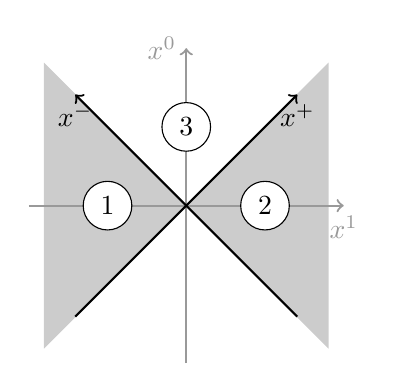
\begin{tikzpicture}
%light cone
\filldraw[black!20] (-1.8,1.8) -- (-1.8,-1.8) -- (1.8,1.8)  -- (1.8,-1.8) -- cycle;
%axes
\draw[->,gray!80,thick] (-2,0) -- (2,0) node[below] {$x^1$};
\draw[->,gray!80,thick] (0,-2) -- (0,2) node[left] {$x^0$}; 
\draw[->,thick] (1.41,-1.41) -- (-1.41,1.41) node[below] {$x^-$};
\draw[->,thick] (-1.41,-1.41) -- (1.41,1.41) node[below] {$x^+$};
%text
\draw (0,1) node[circle,fill=white,draw=black] {$3$};
\draw (-1,0) node[circle,fill=white,draw=black] {$1$};
\draw (1,0) node[circle,fill=white,draw=black] {$2$};
\end{tikzpicture}
	\caption{Partition of spacetime into light-cone quadrants. The quadrants where the Yang-Mills equations will be solved are identified as quadrants 1, 2 and 3. Adapted from \citep{Kovner_1995}.}
	\label{fig:space_partition}
	\end{subfigure}
	\hfill
	\begin{subfigure}{0.55\textwidth}
	\centering
	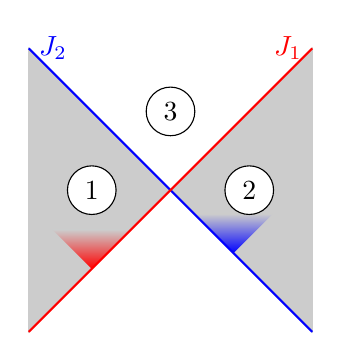
\begin{tikzpicture}
%light cone
\filldraw[black!20] (-1.8,1.8) -- (-1.8,-1.8) -- (1.8,1.8)  -- (1.8,-1.8) -- cycle;

%lightcones
\shade[bottom color=red, top color=black!20] (-1,-1) -- (-0.5,-0.5) -- (-1.5,-0.5) -- cycle;
\shade[bottom color=blue, top color=black!20] (0.8,-0.8) -- (0.3,-0.3) -- (1.3,-0.3) -- cycle;

%\shade[bottom color=red, top color=transparent] (0.3,0.3) -- (0.8,0.8) -- (-0.2,0.8) -- cycle;
%\shade[bottom color=blue] (-0.2,0.2) -- (0.3,0.7) -- (-0.7,0.7) -- cycle;

%axes
%\draw[->,gray!80,thick] (-2,0) -- (2,0) node[below] {$x^1$};
%\draw[->,gray!80,thick] (0,-2) -- (0,2) node[left] {$x^0$}; 
\draw[thick,blue] (1.8,-1.8) -- (-1.8,1.8) node[right] {$J_2$};
\draw[thick,red] (-1.8,-1.8) -- (1.8,1.8) node[left] {$J_1$};



%text
\draw (0,1) node[circle,fill=white,draw=black] {$3$};
\draw (-1,0) node[circle,fill=white,draw=black] {$1$};
\draw (1,0) node[circle,fill=white,draw=black] {$2$};
\end{tikzpicture}
	\caption{The same four quadrants with the support of current $J_1$ ($J_2$) drawn as a red (blue) line. Future light-cones drawn from points where $J_1$ passes only occupy quadrants 1 and 3; future light-cones drawn from points where $J_2$ passes only occupy quadrants 2 and 3.}
	\label{fig:current_light-cones}
	\end{subfigure}
	\caption{}
\end{figure}

For the purpose of solving the Yang-Mills equations, spacetime is divided into four quadrants in $(x^+,x^-)$ space,  as illustrated in Fig. \ref{fig:space_partition}. Quadrants 1 and 2 are named the pre-collision quadrants, while quadrant 3, where the glasma will be described, is referred to as the forward light-cone. For calculations in the third quadrant, the Milne coordinate system\footnote{Also called the Bjorken or Comoving coordinate system.} is used, where positions and four-vectors are given by:
\begin{subequations}
\begin{gather}
	\tau = \sqrt{2x^+x^-} \\
	\eta = \frac{1}{2} \log \left( \frac{x^+}{x^-} \right)
\end{gather}
\end{subequations}
\begin{subequations}
\begin{align}
A^\tau & = \frac{x^- A^+ + x^+ A^-}{\tau} \\
A^\eta & = \frac{x^- A^+ - x^+ A^-}{\tau^2} \label{eq:milne_Aeta}
\end{align}
\end{subequations}
and the transverse components ($i=2,3$) keep their Cartesian form. $\tau$ is called the proper time and $\eta$ is called the rapidity. For a more detailed overview of the Milne coordinates, see Appendix \ref{ap:bjorken_coordinates}.

Drawing future light-cones out from points where the color currents pass in $(x^+,x^-)$ space, one notices that all points in quadrant 1 may not be affected by the $J_2$ current, due to causality; in the same manner, all points in quadrant 2 may not be affected by current $J_1$. Only points in quadrant 3 are causally related to both currents (Fig. \ref{fig:current_light-cones}). Following \cite{Albacete_2019}'s approach, this permits the ``single-nuclei" results of the previous section to be used for the gluon fields in quadrants 1 and 2, reducing the problem to solving the Yang-Mills equations in the third quadrant. Even though they were obtained using different gauge conditions ($A^+ = 0$ for the first nucleus and $A^- = 0$ for the second nucleus), the result in Eqs. (\ref{eq:A_lc_one_nucleus}) and (\ref{eq:A^i_factorization}) can be used for the fields in quadrant 1 and the result in Eqs. (\ref{eq:A_lc_one_nucleus_2}) can be used for the fields in quadrant 2, since those regions are not causally related. In solving the Yang Mills equations for the case of two nuclei, the Fock-Schwinger gauge is chosen, defined by the axial gauge condition:
\begin{equation}
	x^+ A^- + x^- A^+ = 0 ~ \Leftrightarrow ~ A^\tau = 0
\end{equation}
which is obeyed by the solutions built for quadrants 1 and 2. Moving on to quadrant 3, in its interior, this gauge choice requires $A^+$ and $A^-$ to be related as:
\begin{equation}
	A^- = -\frac{x^-}{x^+} A^+ 
\end{equation}
which suggests the definition of an $\alpha$ field as:
\begin{equation}
	A^+ \equiv x^+ \alpha \implies A^- = - x^- \alpha
\end{equation}
Inserting these definitions in Eq. (\ref{eq:milne_Aeta}), the $\alpha$ field can be shown to be equal to $A^\eta$.

Following the ansatz first proposed in \cite{Kovner_1995}, the $\alpha$ field and the transverse fields of the third quadrant, $\alpha^i$, are taken not to depend on $\eta$. This is so that the form of the solution in the third quadrant is not altered by applying a boost to the studied system along the direction of motion of the two nuclei, since the system is invariant under boosts along the $x^1$ axis. For any boost applied, the two infinitely thin nuclei will keep moving at the speed of light, making the boosted system indistinguishable from the original and requiring a solution of the same form. Compiling all the information gathered so far regarding the form of the solution,
\begin{subequations}
\begin{alignat}{2}
& A^+ (x^\mu) &&= \underbrace{\theta (x^+) \theta(x^-)}_{\Circled{3}} x^+ \alpha (\tau, \mathbf{x}_\perp)\\
& A^- (x^\mu) &&= - \underbrace{\theta (x^+) \theta(x^-)}_{\Circled{3}} x^- \alpha (\tau, \mathbf{x}_\perp) \\
& A^{i}(x^\mu) &&= \underbrace{\theta (-x^+) \theta(x^-)}_{\Circled{1}} \alpha^i_1 (\mathbf{x}_\perp)
 + \underbrace{\theta (x^+) \theta(-x^-)}_{\Circled{2}} \alpha^i_2 (\mathbf{x}_\perp)
 + \underbrace{\theta (x^+) \theta(x^-)}_{\Circled{3}} \alpha^i (\tau, \mathbf{x}_\perp)
\end{alignat}
\label{eq:ansatz}
\end{subequations}
%\textcolor{red}{Attention: \citep{Kovner_1995} initially posits that $A^+$ and $A^-$ are different}
For the third quadrant (terms underbraced with `3'), applying such a boost as described leaves the form of the solution unchanged, as $\tau$ and $\mathbf{x}_\perp$ are invariant under it. % \textcolor{purple}{Specify why the $A^+$ and $A^-$ terms are invariant?}

In the interior of the third quadrant, the currents $J_1^\mu$ and $J_2^\mu$ (Eq. \ref{eq:full_J}) have no support, and the Yang-Mills equations take the form:
\begin{equation}
	[D_\mu, F^{\mu\nu}] = 0
\end{equation}

%Before moving on to their treatment, a discussion of the boundary conditions to be used to connect the solution in the forward light-cone with the already-found solutions in the pre-collision quadrants is in order. It is possible to obtain, out of the already-found fields in the pre-collision quadrants, boundary conditions along the edges of the forward light-cone. A detailed derivation of these boundary conditions may be found in \cite[Appendix C]{Carrington_2022_Energy_Momentum_Tensor}. They are obtained by first considering that the longitudinal width of the sources is finite and greater than 0, rather than infinitely thin as in Eq. (2.32), then integrating the Yang-Mills equations over a path (Eq. (\ref{eq:boundary_alpha})) and an area (Eq. (\ref{eq:boundary_transverse})) which cross the light-cone, and finally taking the limit where the width goes to zero. They are:
Before moving on to their treatment, a discussion of the boundary conditions to be used to connect the solution in the forward light-cone with the found solutions in the pre-collision quadrants is in order. It is possible to obtain, out of the found fields in the pre-collision quadrants, starting values for the fields in the forward light-cone at $\tau = 0^+$. This is usually done by requiring that, using the ansatz in Eq. (\ref{eq:ansatz}), the Yang-Mills equations be regular at $\tau = 0$ \cite{Guerrero_Rodr_guez_2021}. They may also be obtained by first considering that the longitudinal width of the sources is finite and greater than $0$, rather than infinitely thin as in Eq. (\ref{eq:thin_rho}), then integrating the Yang-Mills equations over a path (Eq. (\ref{eq:boundary_alpha})) and an area (Eq. (\ref{eq:boundary_transverse})) which cross the light-cone, and finally taking the limit where the width of the sources goes to zero. \cite[Appendix C]{Carrington_2022_Energy_Momentum_Tensor} The obtained boundary conditions are:
\begin{subequations}
\label{eq:boundary_conditions}
\begin{align}
	\alpha(\tau \to 0^+, \mathbf{x}_\perp) & = \frac{ig}{2} \left[ \alpha_1^i(\mathbf{x}_\perp), \alpha_2^i(\mathbf{x}_\perp) \right]
	\label{eq:boundary_alpha} \\
	\alpha^i(\tau \to 0^+, \mathbf{x}_\perp) & =  \alpha_1^i(\mathbf{x}_\perp) + \alpha_2^i(\mathbf{x}_\perp)
	\label{eq:boundary_transverse}
\end{align}
\end{subequations}

Another way to express these boundary conditions is via the chromodynamic force fields: the electric chromodynamic field, $\mathbf{E}$, and the magnetic chromodynamic field, $\mathbf{B}$, which will be referred to simply as the electric and magnetic fields. In Minkowski coordinates, the components of the chromodynamic fields are obtained from the components of the gluon field strength tensor, $F^{\mu \nu}$, following \cite{Lappi:2017skr}, as:
\begin{subequations}
\begin{gather}
E^i = F_{0 i}\\
B^i = -\frac12 \varepsilon^{ijk} F_{jk}
\end{gather}
\end{subequations}
with $i,j,k=1,2,3$, as in the case of Classical Electrodynamics. In Milne coordinates, the components are defined as:
\begin{subequations}
\begin{alignat}{2}
E^\eta &= \frac{1}{\tau} F_{\tau \eta}  = - F_{+ -}
 && E^i = F_{\tau i} \label{eq:E_from_F} \\
 B^\eta &= -\frac12 \varepsilon^{ij} F_{ij} = -F_{23} \quad
&& B^i = -\varepsilon^{ij} \frac{1}{\tau} F_{j \eta} \label{eq:B_from_F}
\end{alignat}
\label{eq:E_B_from_F}
\end{subequations}
with $i,j=2,3$. Defined this way, $E^\eta= E^1$ and $B^\eta = B^1$ everywhere, earning them the name ``longitudinal fields''; on the other hand, $E^i_{\text{Minkowski}} = E^i_{\text{Milne}}$  and $B^i_{\text{Minkowski}} = B^i_{\text{Milne}}$ ($i=2,3$) at midrapidity -- these are the transverse chromodynamic fields.

The boundary conditions for the electric and magnetic fields  are obtainable by calculating the relevant components of $F^{\mu \nu}$ using the boundary conditions already found for $\alpha$ and $\alpha^i$ (Eqs. (\ref{eq:boundary_conditions})):
\begin{subequations}
\begin{gather}
E^\eta_0 (\mathbf{x}_\perp) = - ig \delta^{ij} \left[ \alpha_1^i(\mathbf{x}_\perp), \alpha_2^j(\mathbf{x}_\perp) \right] 
\label{eq:E_from_precollision}\\
B^\eta_0 (\mathbf{x}_\perp) = -ig \varepsilon^{ij} \left[ \alpha_1^i(\mathbf{x}_\perp), \alpha_2^j(\mathbf{x}_\perp) \right]
\label{eq:B_from_precollision}
\end{gather}
\label{eq:EB_from_precollision}
\end{subequations}
Additionally, the initial chromodynamic fields are purely longitudinal; that is, the transverse fields are initially null, $E^i_0 = B^i_0 = 0$ (the steps of this derivation are detailed in Appendix \ref{ap:EB_from_precollision}). The absence of initial transverse fields motivates the ``glasma flux tube'' picture of the early glasma, which is illustrated in Fig. \ref{fig:flux_tubes}. 
\begin{figure}
    \centering    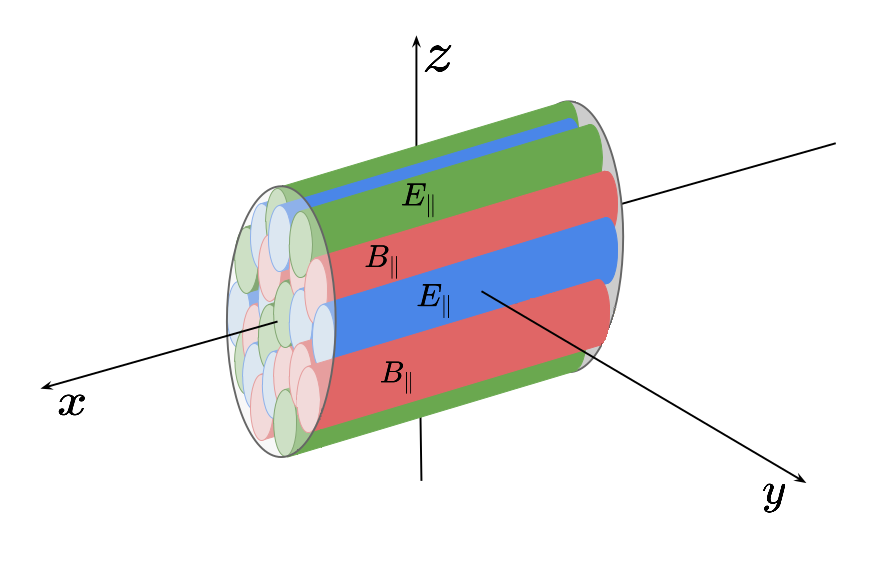
\includegraphics[width=0.6\textwidth]{Figures/flux_tubes.png}
    \caption{The ``glasma flux tube'' picture of the early glasma ($\tau \to 0^+$). Right after the collision, the space between the receding nuclei is populated by purely longitudinal chromoelectric and chromomagnetic fields, whose direction lies along the drawn tubes. Adapted from \cite{Carrington_2022}.}
    \label{fig:flux_tubes}
\end{figure} 

Moving on to the treatment of the Yang-Mills equations, defining $Y^\nu \equiv [D_\mu, F^{\mu\nu}]$, the $\tau$ and $\eta$ components of the system of equations in comoving coordinates may be obtained out of the $+$ and $-$ components in light-cone coordinates as:
\begin{subequations}
\begin{gather}
	Y^\tau = 0 ~ \Leftrightarrow ~ \frac{x^- Y^+ + x^+ Y^-}{\tau} = 0 \\
	Y^\eta = 0 ~ \Leftrightarrow ~ \frac{x^- Y^+ - x^+ Y^-}{\tau^2} = 0
\end{gather}
\end{subequations}
and the $\nu = 2,3$ components keep their cartesian form.

Inserting Eq. (\ref{eq:ansatz}) into the Yang-Mills equations in comoving coordinates returns:
\begin{subequations}
\begin{align}
	& Y^\tau = 0 \quad \Leftrightarrow \quad ig\tau \left[\alpha, \partial_\tau \alpha \right] - \frac{1}{\tau} \left[D_i, \partial_\tau \alpha^i \right] = 0 \\
	& Y^\eta = 0 \quad \Leftrightarrow \quad \frac{1}{\tau} \partial_\tau \left( \frac{1}{\tau} \partial_\tau \left( \tau^2 \alpha \right) \right) - \left[D^i, \left[D^i, \alpha \right] \right] = 0 \\
	& Y^i = 0 \quad \Leftrightarrow \quad \frac{1}{\tau} \partial_\tau \left( \tau \partial_\tau \alpha^i \right) - ig\tau^2 \left[\alpha, \left[D^i,\alpha \right] \right] - [D^j, F^{ji}] = 0
\end{align}
\end{subequations}
where $i,j=2,3$.

These equations have no known analytical solution, but have been studied numerically and analytically via approximations. In this work, the approximation that will allow the analytical treatment of the equations is their linearization; that is, the neglect of second or higher order terms in the fields
%, which was first done in \cite{}
. This  will naturally do away with gauge invariance, as the value of the neglected terms changes according to the used gauge. Therefore, one must choose the proper gauge, which minimizes the influence of these terms, before linearizing the equations. Two criteria are put forward in \cite{Guerrero_Rodr_guez_2021}: keeping the result independent of $\eta$ suggests that the gauge transformation matrix should be independent of $\eta$ as well; additionally, since there are no color charge sources in the interior of the forward light-cone that would generate a static Coulomb field,
the Fock-Schwinger gauge condition ($A^\tau = 0$) is maintained\footnote{Maintaining the Fock-Schwinger gauge also ensures that $A^-$ remains $0$ in the support of the right-moving current and $A^+$ remains $0$ in the support of the left-moving current, doing away with the complicated Wilson Line operators that would be needed to ensure their covariant conservation.}, which can be achieved by requiring the gauge transformation to be independent of $\tau$. Thus, the inverse gauge transformation is:
\begin{subequations}
\begin{gather}
	\alpha(\tau,\mathbf{x}_\perp) = V (\mathbf{x}_\perp) \beta(\tau,\mathbf{x}_\perp) V^\dagger (\mathbf{x}_\perp) \\
	\alpha^i(\tau,\mathbf{x}_\perp) = V (\mathbf{x}_\perp) \left( \beta(\tau,\mathbf{x}_\perp) - \frac{1}{ig} \partial^i \right) V^\dagger (\mathbf{x}_\perp)
\end{gather}
\end{subequations}
which makes the linearized Yang-Mills equations for the fields in the new gauge, 
%\textcolor{purple}{CHECK}
\begin{subequations}
\begin{gather}
	\partial_\tau \partial_i \beta^i = 0 \\
	\frac{1}{\tau} \partial_\tau \left( \frac{1}{\tau} \partial_\tau \left( \tau^2 \beta \right) \right) - \partial^{\textcolor{purple}{i}} \partial^i \beta = 0 \\
	\frac{1}{\tau} \partial_\tau \left( \tau \partial_\tau \beta^i \right) - \left( \partial^k \partial^{\textcolor{purple}{k}} \delta^{i j} - \partial^j \partial^i \right) \beta^j =0
\end{gather}
\end{subequations}
where $k=2,3$. %(\textcolor{purple}{different signs in 1808 and 2102})

The remaining gauge freedom allows setting $\partial_i \beta^i = 0$, a Coulomb gauge condition, minimizing the amplitudes of the transverse fields \cite{Blaizot:2010kh}. The equations become:
\begin{subequations}
\begin{gather}
	\partial_\tau \left( \frac{1}{\tau} \partial_\tau \left( \tau^2 \beta \right) \right) - \tau \partial^{\textcolor{purple}{i}}  \partial^i \beta = 0 \\
	\partial_\tau \left( \tau \partial_\tau \beta^i \right) - \tau \partial^k \partial^{\textcolor{purple}{k}} \beta^i =0
\end{gather}
\end{subequations}

Taking the transverse position Fourier transform on both sides,
\begin{subequations}
\begin{gather}
	\beta (\tau, \mathbf{x}_\perp) = \iint \frac{\diff^2 \mathbf{k}_\perp}{(2\pi)^2} ~ e^{i (k_\perp)^j (x_\perp)_j} \tilde{\beta} (\tau, \mathbf{k}_\perp) \\
	\beta^i (\tau, \mathbf{x}_\perp) = \iint \frac{\diff^2 \mathbf{k}_\perp}{(2\pi)^2} ~ e^{i (k_\perp)^j (x_\perp)_j} \tilde{\beta}^i (\tau, \mathbf{k}_\perp)
\end{gather}
\end{subequations}
the equations for $\tilde{\beta}$ and $\tilde{\beta}^i$ are:
\begin{subequations}
\begin{gather}
	\tau^2 \partial_\tau^2 \big(\tau \tilde{\beta}\big) + \tau \partial_\tau \big(\tau \tilde{\beta}\big) + \big(\tau^2 k^2 - 1\big) \big(\tau \tilde{\beta}\big) = 0  \label{eq:bessel_beta}\\ 
	\tau^2 \partial_\tau^2 \tilde{\beta}^i + \tau \partial_\tau \tilde{\beta}^i + \tau^2 k^2  \tilde{\beta}^i =0 \label{eq:bessel_beta_i}
\end{gather}
\end{subequations}
where $k\equiv |\mathbf{k}_\perp| = \sqrt{(k^2)^2+(k^3)^2}$ is the Euclidean norm of $\mathbf{k}_\perp$.

%In order to simplify the expressions, $\omega$ is defined as $\omega \equiv |\mathbf{k}_\perp|  \equiv \sqrt{(k^2)^2+(k^3)^2}$.

Once the change of variable $z= k \tau$ is made, Eq. (\ref{eq:bessel_beta}) is a Bessel differential equation of degree 1 for the function $\tau \tilde{\beta}$. It admits as solutions linear combinations of the Bessel functions of order 1 of the first and second kind, $J_1(k \tau)$ and $Y_1(k \tau)$. Similarly, after the same change of variable, Eq. (\ref{eq:bessel_beta_i}) is a Bessel differential equation of degree 0 for the function $\tilde{\beta}^i$, which admits as solutions linear combinations of the Bessel functions of order 0 of the first and second kind, $J_0(k \tau)$ and $Y_0(k \tau)$. \cite{arfken2005mathematical} As the Bessel functions of the second kind, $Y_n$, are singular at the origin for integer $n$, they are taken as unphysical solutions and their coefficients are set to $0$. 

The solution is, then,
\begin{subequations}
\begin{align}
	\tilde{\beta} (\tau, \mathbf{k}_\perp) &= \tilde{\beta}_0 (\mathbf{k}_\perp) \frac{2 J_1(k \tau)}{k \tau} \label{eq:beta_tilde}\\
	\tilde{\beta}^i (\tau, \mathbf{k}_\perp) &= \tilde{\beta}^i_0 (\mathbf{k}_\perp) J_0(k \tau) \label{eq:beta^i_tilde}
\end{align}
\end{subequations}
where the factor of $2$ in Eq. (\ref{eq:beta_tilde}) was introduced in order to make the $\mathbf{k}_\perp$-dependent coefficient, $\tilde{\beta}_0$, match the value of $\tilde{\beta}$ at $\tau=0$, since $\lim_{z \to 0} J_1(z)/z=1/2$. \cite{arfken2005mathematical}

In order to find the expressions for the fields at $\tau = 0$ ($\tilde{\beta}_0$ and $\tilde{\beta}^i_0$), the next step would be to use the boundary conditions of Eqs. (\ref{eq:boundary_conditions}), which would require first bringing the pre-collision potentials, $\alpha^i_1$ and $\alpha^i_2$, to the Coulomb gauge. No analytical expression for the necessary transformation matrix $V(\mathbf{x}_\perp)$ has been found; however, solving the linearized equations using numerically-computed boundary conditions in the Coulomb gauge has been found to approximate the resolution of the full Yang-Mills equations quite well \cite{Guerrero_Rodr_guez_2021,Blaizot:2010kh}%\textcolor{purple}{(read paper, quantify similarity)}
, except for very soft modes (very low $|\mathbf{k}_\perp|$). %\textcolor{purple}{(quantify)}

One way to go around this problem is to recall that the quantities needed to compute the physically meaningful results are the chromodynamic force fields: the electric field, $\mathbf{E}$, and the magnetic field, $\mathbf{B}$. They will be used to calculate color traces of products of their components, like $\Tr_c [E^i(\tau, \mathbf{x}_\perp) B^j(\tau', \mathbf{y}_\perp) ]$, for example. Checking for gauge invariance, since the field components change under the transformation to the Coulomb gauge as $E^i (\tau, \mathbf{x}_\perp) \to E'^i(\tau, \mathbf{x}_\perp) = V(\mathbf{x}_\perp) E^i(\tau, \mathbf{x}_\perp) V^\dagger(\mathbf{x}_\perp)$ %\textcolor{purple}{(NOT GAUGE INVARIANT FOR $v_\perp \neq 0$ ??
% But maybe $\hat{q}$ and $dE/dx$ are)
, the previous trace is gauge invariant. 

As such, in order to obtain the initial fields $\tilde{\beta}_0$ and $\tilde{\beta}_0^i$, one may choose them so as to produce the appropriate initial chromodynamic fields given by Eqs. (\ref{eq:EB_from_precollision}): $\mathbf{E}_0 (\mathbf{x}_\perp) \equiv \mathbf{E}(\tau \to 0^+,\mathbf{x}_\perp)$ and \linebreak $\mathbf{B}_0 (\mathbf{x}_\perp) \equiv \mathbf{B}(\tau \to 0^+,\mathbf{x}_\perp)$.

The relations between the initial gluon fields and the initial chromodynamic fields are obtained from taking the Fourier transform of the gluon and chromodynamic fields in Eqs. (\ref{eq:E_B_from_F}), as detailed in Appendix \ref{ap:betas_and_EBs}:
\begin{subequations}
\begin{align}
\label{eq:betas_and_E}
\tilde{E}_0^\eta (\mathbf{k}_\perp) = -2 \tilde{\beta}_0 (\mathbf{k}_\perp) & \implies \tilde{\beta}_0 (\mathbf{k}_\perp) = -\frac12 \tilde{E}_0^\eta (\mathbf{k}_\perp)\\ 
\label{eq:betas_and_B}
\tilde{B}_0^\eta (\mathbf{k}_\perp) = - i \varepsilon^{ij} k^i \tilde{\beta}_0^j (\mathbf{k}_\perp) & \implies \tilde{\beta}^i_0 (\mathbf{k}_\perp)= - i \varepsilon^{ij} \frac{k^j}{|\mathbf{k}_\perp|^2} \tilde{B}_0^\eta(\mathbf{k}_\perp) 
\end{align}
\label{eq:betas_and_EBs}
\end{subequations}
%\tilde{E}_0^i = \\
%\tilde{B}_0^i =

Thus, the chain of expressions which allows writing the chromodynamic fields as functions of the pre-collision potentials is now complete.
\begin{subequations} \label{eq:EB_from_initial_EB}
\begin{align}
\tilde{E}^\eta(\tau,\mathbf{k}_\perp) & = \tilde{E}^\eta_0 (\mathbf{k}_\perp) J_0 (k \tau) \\
\tilde{E}^i(\tau,\mathbf{k}_\perp) & = -i \varepsilon^{ij} (k^j/k) \tilde{B}_0^\eta (\mathbf{k}_\perp) J_1 (k \tau) \\
\tilde{B}^\eta(\tau,\mathbf{k}_\perp) & = \tilde{B}^\eta_0 (\mathbf{k}_\perp) J_0 (k \tau) \\
\tilde{B}^i(\tau,\mathbf{k}_\perp) & = \textcolor{red}{-}i \varepsilon^{ij} (k^j/k) \tilde{E}_0^\eta (\mathbf{k}_\perp) J_1 (k \tau)
\end{align}
\end{subequations}

In order to obtain these expressions in position space, it is necessary to calculate the Fourier transforms of Eqs. (\ref{eq:EB_from_precollision}) to insert into Eqs. (\ref{eq:EB_from_initial_EB}), before applying the Fourier transform again to finish at position space. For example, for $E^i$:

\begin{subequations}
\label{eq:chromodynamic_fields_full}
\begin{align}
\begin{split}
	E^i (\tau,\mathbf{x}_\perp) & =  \int \frac{\diff^2 \mathbf{k}_\perp}{(2\pi)^2} e^{i \mathbf{k}_\perp \cdot \mathbf{x}_\perp} (-i)   \varepsilon^{i j} \frac{k^j}{k} J_1 (k \tau)  \int \diff^2 \mathbf{u}_\perp e^{-i \mathbf{k}_\perp \cdot \mathbf{u}_\perp} (-ig) \varepsilon^{mn} [\alpha^m_{1} (\mathbf{u}_\perp) \alpha^n_{2}(\mathbf{u}_\perp)] \\
	& = -ig \varepsilon^{mn} f^{abc} T_c \varepsilon^{ij} \int  \frac{\diff^2 \mathbf{k}_\perp}{(2\pi)^2} \frac{k^j}{k} J_1 (k \tau) \int \diff^2 \mathbf{u}_\perp e^{i \mathbf{k}_\perp \cdot (\mathbf{x} - \mathbf{u})_\perp} \alpha^m_{1a} (\mathbf{u}_\perp) \alpha^n_{2b}(\mathbf{u}_\perp)
\end{split} \\
\intertext{where the definition $\alpha_i^m(\mathbf{u}_\perp) \equiv \alpha_{ia}^m(\mathbf{u}_\perp) T_a$ and the SU(3) commutation relations, $[T_a,T_b] = if^{abc} T_c$, were used. The remaining components are:}
	E^\eta (\tau,\mathbf{x}_\perp) & = g \delta^{mn} f^{abc} T_c \int  \frac{\diff^2 \mathbf{k}_\perp}{(2\pi)^2} J_0 (k \tau) \int \diff^2 \mathbf{u}_\perp e^{i \mathbf{k}_\perp \cdot (\mathbf{x} - \mathbf{u})_\perp} \alpha^m_{1a} (\mathbf{u}_\perp) \alpha^n_{2b}(\mathbf{u}_\perp) \\
	B^\eta (\tau,\mathbf{x}_\perp) & = g \varepsilon^{mn} f^{abc} T_c \int  \frac{\diff^2 \mathbf{k}_\perp}{(2\pi)^2} J_0 (k \tau) \int \diff^2 \mathbf{u}_\perp e^{i \mathbf{k}_\perp \cdot (\mathbf{x} - \mathbf{u})_\perp} \alpha^m_{1a} (\mathbf{u}_\perp) \alpha^n_{2b}(\mathbf{u}_\perp) \\
	B^i (\tau,\mathbf{x}_\perp) & = -ig \delta^{mn} f^{abc} T_c \varepsilon^{i j} \int  \frac{\diff^2 \mathbf{k}_\perp}{(2\pi)^2} \frac{k^j}{k} J_1 (k \tau) \int \diff^2 \mathbf{u}_\perp e^{i \mathbf{k}_\perp \cdot (\mathbf{x} - \mathbf{u})_\perp} \alpha^m_{1a} (\mathbf{u}_\perp) \alpha^n_{2b}(\mathbf{u}_\perp)
\end{align}
\end{subequations}

These expressions are quite lengthy. However, they may be more easily treated remembering their shared  structure. For a general chromodynamic field $G^\alpha (\tau, \mathbf{x}_\perp)$, with $\alpha = \eta,2,3$:

\begin{equation}
\label{eq:shared_structure}
 G^\alpha (\tau, \mathbf{x}_\perp) = C^{mn} ~ g f^{abc} T_c \int  \frac{\diff^2 \mathbf{k}_\perp}{(2\pi)^2} ~ D^\alpha (\tau, \mathbf{k}_\perp) \int \diff^2 \mathbf{u}_\perp e^{i \mathbf{k}_\perp \cdot (\mathbf{x} - \mathbf{u})_\perp} \alpha^m_{1a} (\mathbf{u}_\perp) \alpha^n_{2b} (\mathbf{u}_\perp)
\end{equation}
where $D^\eta = J_0(k \tau)$  and, for $i=2,3$, $D^i = -i \varepsilon^{ij} (k^j/k) J_1(k \tau)$; and  $C^{mn} = \delta^{mn}$ for $E^\eta$ and $B^i$ and $C^{mn} = \varepsilon^{mn}$ for $E^i$ and $B^\eta$.



\begin{comment}
----------------------


%In the case of a HIC, in the center of mass \textcolor{red}{(laboratory?)} frame, two heavy nuclei travel at (close to) the speed of light along the $z$ axis in opposing directions. The nuclei moving in the positive or negative $z$ direction are named nucleus 1 or nucleus 2, respectively.

In light cone coordinates, for nucleus 1, the only non-vanishing component of the color current four-vector $J^\nu$ is the $+$ component, ${J_1}^+$ (see Eq. (\ref{eq:+_Current})); for nucleus 2, by equivalent arguments applied to a nucleus moving in the opposite direction, the only non-vanishing component is the $-$ component, ${J_2}^-$, which has a similar form to ${J_1}^+$, but exchanging $x^- \to x^+$ \textcolor{red}{\footnote{\textcolor{red}{\cite{Carrington_2022_Energy_Momentum_Tensor} \cite{Gelis_Habilitation} allows the nuclei to retain some thickness and then brings it to 0 at the end of the calculation. It justifies the use of $\rho$ as a surface charge density, I think.}}}: \textcolor{blue}{gauge-dependent charge density}
\begin{equation*}
	{J_1}^+ = g \delta (x^-) \rho_1 (\mathbf{x}_\perp) \qquad {J_2}^- = g \delta (x^+) \rho_2 (\mathbf{x}_\perp)
\end{equation*}
where $\rho_{1,2}$ are the static number color densities in nuclei 1 and 2 per unit of transverse area.
%The Lorentz contraction in the $x^1$ direction suffered by nucleus 1 implies a very thin spread of color charge in the $x^-$ direction, so the dependence on this coordinate is factorized as $\delta(x^-)$ \cite{Gelis_Habilitation} \textcolor{blue}{ This reference}; \textcolor{red}{if we consider additionally that, due to length contraction along the $x^1$ direction, the nucleus is infinitely thin, and therefore extends only in the $\mathbf{x}_\perp$ plane, then $\rho_1$ may not depend on $x^+$ either}. Equivalently, for nucleus 2, which travels along the $x^-$ axis, the color charge spread along the $x^+$ direction is factorized into $\delta(x^+)$ \textcolor{red}{and, if considered infinitely thin, neither on $x^-$.}
%where $\rho_{1,2}$ are the static number color densities in nuclei 1 and 2 per unit of transverse area. Since nucleus 1 travels along the $x^+$ axis, its number color density $\rho_1$ may not depend on $x^-$; if we consider additionally that, due to length contraction along the $x^1$ direction, the nucleus is infinitely thin, and therefore extends only in the $\mathbf{x}_\perp$ plane, then $\rho_1$ may not depend on $x^+$ either. Equivalently, for nucleus 2, which travels along the $x^-$ axis, $\rho_2$ may not depend on $x^+$ and, if considered infinitely thin, neither on $x^-$.

Adding the contributions of both color currents, the source term becomes:
\begin{equation}
J^\nu = g \delta^\nu_+ \delta (x^-) \rho_1 (\mathbf{x}_\perp) + g \delta^\nu_- \delta (x^+) \rho_2 (\mathbf{x}_\perp)
\end{equation}

The classical Yang-Mills equations to be solved in the presence of the static color sources become, then,

\begin{equation}
	 [D_\mu, F^{\mu \nu}] = J^\nu
\end{equation}

\end{comment}

\begin{comment}
\section{\textcolor{red}{Transcribed expressions yet without text}}

\begin{subequations} \label{eq:initial_fields}
\begin{equation}
\begin{split}
E^\eta_0(\mathbf{x}_\perp) & = -ig \delta^{ij} [\alpha^i_1 (\mathbf{x}_\perp), \alpha^j_2(\mathbf{x}_\perp)] \\
 & = g \delta^{ij}   \alpha^i_{1a} (\mathbf{x}_\perp) \alpha^j_{2b}(\mathbf{x}_\perp)f^{abc} T_c
\end{split} \label{eq:initial_E}
\end{equation}
\begin{equation}
\begin{split}
B^\eta_0(\mathbf{x}_\perp) & = -ig \varepsilon^{ij} [\alpha^i_1 (\mathbf{x}_\perp), \alpha^j_2(\mathbf{x}_\perp)] \\
& = g \varepsilon^{ij} \alpha^i_{1a} (\mathbf{x}_\perp) \alpha^j_{2b}(\mathbf{x}_\perp) f^{abc} T_c
\end{split} \label{eq:initial_B}
\end{equation}
\end{subequations}


In order to get expressions for one of the fields in coordinate  space\textcolor{red}{\footnote{as is necessary in order to calculate $X^{\alpha \beta}$}}, the appropriate field at $\tau=0^+$ (eqs. \ref{eq:initial_fields}) must be Fourier-transformed and used in Eqs. (\ref{eq:EB_from_initial_EB}). The inverse Fourier transform is then applied to the resulting expression. For $E^\alpha$, $\alpha=2,3$, for example:

\begin{equation}
\begin{alignedat}{2}
	E^\alpha (\tau,\mathbf{x}_\perp) & =  \int \frac{\diff^2 \mathbf{k}_\perp}{(2\pi^2)} e^{i \mathbf{k}_\perp \cdot \mathbf{x}_\perp} & & (-i)   \varepsilon^{\alpha \beta} \hat{k}^\beta J_1 (k \tau)  \int \diff^2 \mathbf{u}_\perp e^{-i \mathbf{k}_\perp \cdot \mathbf{u}_\perp} \\
	& ~ & & \times ~ g \varepsilon^{ij} \alpha^i_{1a} (\mathbf{u}_\perp) \alpha^j_{2b}(\mathbf{u}_\perp) f^{abc} T_c \\
	& = -ig \varepsilon^{ij} f^{abc} T_c \varepsilon^{\alpha \beta} & & \int  \frac{\diff^2 \mathbf{k}_\perp}{(2\pi^2)} \hat{k}^\beta J_1 (k \tau) \int \diff^2 \mathbf{u}_\perp e^{i \mathbf{k}_\perp \cdot (\mathbf{x} - \mathbf{u})_\perp}  \\
	& ~ & & \times \alpha^i_{1a} (\mathbf{u}_\perp) \alpha^j_{2b}(\mathbf{u}_\perp)
\end{alignedat}
\end{equation}

And the remaining fields:

\begin{align}
	E^\eta (\tau,\mathbf{x}_\perp) & = g \delta^{ij} f^{abc} T_c \int  \frac{\diff^2 \mathbf{k}_\perp}{(2\pi^2)} J_0 (k \tau) \int \diff^2 \mathbf{u}_\perp e^{i \mathbf{k}_\perp \cdot (\mathbf{x} - \mathbf{u})_\perp} \alpha^i_{1a} (\mathbf{u}_\perp) \alpha^j_{2b}(\mathbf{u}_\perp) \\
	B^\eta (\tau,\mathbf{x}_\perp) & = g \varepsilon^{ij} f^{abc} T_c \int  \frac{\diff^2 \mathbf{k}_\perp}{(2\pi^2)} J_0 (k \tau) \int \diff^2 \mathbf{u}_\perp e^{i \mathbf{k}_\perp \cdot (\mathbf{x} - \mathbf{u})_\perp} \alpha^i_{1a} (\mathbf{u}_\perp) \alpha^j_{2b}(\mathbf{u}_\perp) \\
	B^\alpha (\tau,\mathbf{x}_\perp) & = -ig \delta^{ij} f^{abc} T_c \varepsilon^{\alpha \beta} \int  \frac{\diff^2 \mathbf{k}_\perp}{(2\pi^2)} \hat{k}^\beta J_1 (k \tau) \int \diff^2 \mathbf{u}_\perp e^{i \mathbf{k}_\perp \cdot (\mathbf{x} - \mathbf{u})_\perp} \alpha^i_{1a} (\mathbf{u}_\perp) \alpha^j_{2b}(\mathbf{u}_\perp)
\end{align}
\end{comment}

\section{The two-point gluon field correlator}

%\textcolor{purple}{How is this form for the correlator justified? $G(|\mathbf{x}_\perp - \mathbf{y}_\perp|, \mathbf{x}_\perp + \mathbf{y}_\perp )$ is symmetric! Could there be any more arguments for the $G$ function?}

%The previous section has ended with expressions for the chromodynamic fields $\mathbf{E}$ and $\mathbf{B}$ out of the gluon fields $\alpha$. In the next chapter, the procedure for extracting macroscopic information about the pre-hydrodynamic stage will be presented, and it will require the calculation of chromodynamic field correlators

The two-point gluon field correlator will be a useful quantity for Chapter \ref{ch:merge}, and it is computable within the present formalism. The correlator,
\begin{equation}
	\left< \alpha^i_{pa} (\mathbf{x}_\perp) \alpha^j_{qb} (\mathbf{y}_\perp) \right>
\end{equation}
should be $0$ for gluon fields from different nuclei, $p \neq q$, as they are causally unrelated, and for different colors, $a \neq b$ \cite{Lappi:2017skr}.


A general form for the correlator in heavy ion collisions is: \cite{Lappi:2017skr}
\begin{equation}
	\left< \alpha^i_{pa} (\mathbf{x}_\perp) \alpha^j_{qb} (\mathbf{y}_\perp) \right> = 
	 \delta^{pq}\delta^{ab} \frac{1}{2}
	\left( \delta^{ij} G_p (\mathbf{x}_\perp,\mathbf{y}_\perp) + \left(\delta^{ij} - 2 \frac{r^i r^j}{r^2} \right) h_p (\mathbf{x}_\perp,\mathbf{y}_\perp) \right)
\label{eq:general_correlator}
\end{equation}
where $\mathbf{r} \equiv \mathbf{x}_\perp - \mathbf{y}_\perp$, and $G$ and $h$ are called the unpolarized and polarized gluon distributions, respectively.\footnote{$G$ and $h$ are actually the Hankel transforms of the unpolarized and polarized gluon distributions, $\tilde{G}\big((\mathbf{x}_\perp + \mathbf{y}_\perp)/2,k\big)$  and $\tilde{h}\big((\mathbf{x}_\perp + \mathbf{y}_\perp)/2,k\big)$.}

The product of two correlators, each one for one of the incoming nuclei, will appear further ahead in this work. Defining it as a tensor $C$,
\begin{equation}
 C^{im~jn}_{bd~ce} (\mathbf{x}_\perp,\mathbf{y}_\perp) \equiv \big< \alpha^i_{1b} (\mathbf{x}_\perp) \alpha^m_{1d} (\mathbf{y}_\perp) \big>
 \big< \alpha^j_{2c} (\mathbf{x}_\perp) \alpha^n_{2e} (\mathbf{y}_\perp) \big>
\end{equation}
some of its contractions are:
\begin{subequations}
\begin{align}
\delta^{ij} \varepsilon^{mn} ~
C^{im~jn}_{bd~ce} (\mathbf{x}_\perp,\mathbf{y}_\perp) & = 0 \label{eq:correlator_contractions_null1}\\
\varepsilon^{ij} \delta^{mn} ~
C^{im~jn}_{bd~ce} (\mathbf{x}_\perp,\mathbf{y}_\perp) & = 0 \label{eq:correlator_contractions_null2}\\
\delta^{ij} \delta^{mn} ~
C^{im~jn}_{bd~ce} (\mathbf{x}_\perp,\mathbf{y}_\perp) & = \frac{\delta^{bd}\delta^{ce}}{2} \big( G_1(\mathbf{x}_\perp,\mathbf{y}_\perp) G_2(\mathbf{x}_\perp,\mathbf{y}_\perp) + h_1(\mathbf{x}_\perp,\mathbf{y}_\perp) h_2(\mathbf{x}_\perp,\mathbf{y}_\perp)\big)\\
\varepsilon^{ij} \varepsilon^{mn} ~
C^{im~jn}_{bd~ce} (\mathbf{x}_\perp,\mathbf{y}_\perp) & = \frac{\delta^{bd}\delta^{ce}}{2} \big( G_1(\mathbf{x}_\perp,\mathbf{y}_\perp) G_2(\mathbf{x}_\perp,\mathbf{y}_\perp) - h_1(\mathbf{x}_\perp,\mathbf{y}_\perp) h_2(\mathbf{x}_\perp,\mathbf{y}_\perp)\big)
\end{align}
\label{eq:correlator_contractions}
\end{subequations}
The simple forms of these contractions in terms of $G$ and $h$ functions are the motivation for the separation of the $\delta^{ij}$ and $r^i r^j$ components of the corrrelator as it is done in Eq. (\ref{eq:general_correlator}).

\subsection{In the MV model}

Obtaining the explicit forms of the gluon distributions $G$ and $h$ within the \gls{MV} model requires solving for the $A^+_{(1)}$ field of Eq. (\ref{eq:n_1_A}), renamed field $\Phi$ in Eq. (\ref{eq:A_lc_one_nucleus}). This is done by finding an explicit form for the Green's function:
\begin{equation}
	- \nabla^2_\perp \Phi(x^-, \mathbf{x}_\perp) = g \rho (x^-,\mathbf{x}_\perp) \quad \Rightarrow \quad 
	\Phi(x^-,\mathbf{x}_\perp) = g  \int \diff^2 \mathbf{y}_\perp \mathcal{G}(\mathbf{x_\perp} - \mathbf{y_\perp}) \rho(x^-,\mathbf{y}_\perp)
\end{equation}


The Green's function should obey the equation:
\begin{equation}
	 - \nabla_\perp^2 \mathcal{G} (\mathbf{x}_\perp) = \delta (\mathbf{x}_\perp)
\end{equation}
which is the 2D Poisson's equation for a point color charge, missing a factor of $g$. It is solved in momentum space as\footnote{The 2D inverse Fourier transform of any radial function $\tilde{f}(\mathbf{k}) = \tilde{f}(k)$ is its Hankel transform over $k$, divided by $2 \pi$. The Hankel transform of $1/(k^2 + m^2)$ is given in \cite{Gradshteyn:1943cpj}, integral 6.5324}
\begin{equation}
	 | \mathbf{k}_\perp|^2 \tilde{\mathcal{G}}(\mathbf{k}) = 1 \quad \to \quad \tilde{\mathcal{G}}(\mathbf{k}) = \frac{1}{k^2+m^2} \quad \implies \quad \mathcal{G} (\mathbf{x}_\perp) = \frac{1}{2\pi} K_0 (m |\mathbf{x}_\perp|)
\end{equation}
where $K_0$ is the modified Bessel function of the second kind of degree $0$. The $m$ quantity has been introduced as an infrared ($k \to 0 $) regulator. This procedure is equivalent to modifying the Poisson's equation by adding a gluon mass:
\begin{equation}
	- (\nabla^2_\perp - m^2) \Phi(x^-, \mathbf{x}_\perp) = g \rho (x^-,\mathbf{x}_\perp)
\end{equation}
which screens the color charges, limiting long-distance interactions across the color-charge discs.\footnote{Without the introduction of the infrared regulator, $\mathcal{G}(\mathbf{x}_\perp)$ is proportional to $-\ln |\mathbf{x}_\perp|$, which encodes long-distance interactions. Adding the regulator, $\mathcal{G}(\mathbf{x}_\perp)$ becomes $\frac{1}{2\pi} K_0 (m |\mathbf{x}_\perp|)$, which behaves asymptotically as $\mathcal{G}(\mathbf{x}_\perp \to \infty) \propto e^{-m |\mathbf{x}_\perp|} / \sqrt{m |\mathbf{x}_\perp|}$.} This, effectively, roughly encodes confinement into the solution, an aspect of the Strong Force which would not arise from the Yang-Mills equations on their own. \cite{Carrington_2022,Guerrero_Rodr_guez_2021} Since the characteristic length over which the interaction decays is $1/m$, the value $m = \qty{200}{MeV} \approx \Lambda_{\text{QCD}}$ is chosen.

Using this Green's function, the \gls{MV} model's two-point gluon field correlator may be explicitly calculated, as was done in \cite[Appendix D]{Carrington_2022_Energy_Momentum_Tensor}. If the nucleus in question is given a uniform color charge number distribution, $\mu(\mathbf{x}_\perp) = \mu$, the unpolarized and polarized gluon distributions assume a manageable form. \cite{Carrington_2022,Guerrero_Rodr_guez_2021}\footnote{\cite{Carrington_2022}'s definition of $\mu$ and \cite{Guerrero_Rodr_guez_2021}'s parametrization of the correlator are used here.}
\begin{subequations}
\begin{align}
G_{\text{MV}}(r) & = \frac{g^{2}\mu}{4\pi} ( mrK_{1}(mr) - 2K_{0}(mr) )
~ \frac{1 - \exp \left [\frac{g^{4}\mu N_c}{4\pi m^{2}} (mrK_{1}(mr) - 1) \right ]}{\frac{g^{4}\mu N_c}{4\pi m^{2}} (mrK_{1}(mr) - 1)} \\
h_{\text{MV}}(r) & = - \frac{g^{2}\mu}{4\pi } mrK_{1}(mr) 
~ \frac{1 - \exp \left [ \frac{g^{4}\mu N_c}{4\pi m^{2}} (mrK_{1}(mr) - 1) \right ]}{\frac{g^{4}\mu N_c}{4\pi m^{2}} (mrK_{1}(mr) - 1)}
\end{align}
\label{eq:unregularized_MV_G_h}
\end{subequations}
where $\mathbf{r}_\perp \equiv \mathbf{x}_\perp - \mathbf{y}_\perp$ and $ r \equiv |\mathbf{r}_\perp|$.

%Due to the $K_0 (mr)$ factor, $G_{\text{MV}}$ diverges in the ultraviolet limit ($r \to \infty$), and so must be regularized. 
In the ultraviolet limit ($r \to 0$), the fractions at the r.h.s. of Eqs. (\ref{eq:unregularized_MV_G_h}) approach $1$, and so does $mrK_1(mr)$; however, due to the $K_0 (mr)$ term, $G_{\text{MV}}$ diverges logarithmically, and so must be regularized. 
\textcolor{red}{[Ask for help with the DGLAP interpretation]}.

In \cite{Guerrero_Rodr_guez_2021}, $G_\text{MV}$ is regularized by replacing the coupling constant $g$ with a running coupling in $r$: \textcolor{red}{[Ask about $g(\mu)^2$ --  why is the asymptotic value of $g$ the value of $g$ at the scale $\mu$?]}
\begin{equation}
	g(r^2)^2 = \frac{g(\mu)^2}{\ln\left( \frac{4e^{-2\gamma_e-1}}{m^2 r^2} + e\right)}.
\end{equation}
where $\gamma_e$ is the Euler-Mascheroni constant and $g(\mu)^2$ is the asymptotic squared coupling constant. For both $G_\text{MV}$ and $h_\text{MV}$, only the overall factor $g^2$ is replaced, leaving the couplings in the rightmost fractions unchanged. Since 
\begin{equation}
2K_0 (mr) - mrK_1(mr) \quad \xrightarrow[r \to 0]{} \quad \ln \left( \frac{4e^{-2\gamma_e-1}}{m^2 r^2} \right)
\end{equation}
the regularized $G_\text{MV}$ approaches $\mu^2/(4 \pi g(\mu)^2)$ in the ultraviolet limit.

%\textcolor{purple}{Mention other possible regularization schemes?}

In order to obtain the expressions for $G_\text{MV}$ and $h_\text{MV}$ to be used in the calculations, $\mu$ should be replaced with a quantity adequate for characterizing the scale of the system. The average number color charge density, $\mu$, is the quantity used to characterize dilute color charge systems, in which it has a well-defined physical meaning. For saturated systems such as the two incoming nuclei, the saturation scale $Q_s$ is used instead. In \cite{Guerrero_Rodr_guez_2021}, it is defined in the present context as the value of $r$ above which the rightmost fractions of Eqs. (\ref{eq:unregularized_MV_G_h}) exhibit non-linear behavior. This is taken to be $r^2 \approx g(\mu)^4 \mu N_c / (4 \pi)$. In \cite{Carrington_2022}, the saturation scale's square is also taken to be proportional to $\mu$, $Q_s^2 \approx g^4 \mu$, with the exact proportionality constant requiring methods beyond the \gls{CGC} to be calculated \textcolor{purple}{(say more?)}. Here, \cite{Carrington_2022}'s expression will be preferred:
%, in order to facilitate comparison with their results. Using the asymptotic value for the coupling constant:
\begin{equation}
Q_s^2 = g(\mu)^4 \mu
\end{equation} 
this will also be used within the rightmost fractions, even though the running coupling prescription has not been applied there.

The expressions for $G_\text{MV}$ and $h_\text{MV}$ to be used become, then,
\begin{subequations}
\begin{align}
G_{\text{MV}}(r) & = \frac{Q_s^2}{4\pi g(\mu)^{2}} \frac{ mrK_{1}(mr) - 2K_{0}(mr) } {\ln\left( \frac{4e^{-2\gamma_e-1}}{m^2 r^2} + e\right)}
~ \frac{1 - \exp \left [\frac{N_c}{4\pi} \frac{Q_s^2}{m^2} (mrK_{1}(mr) - 1) \right ]}{\frac{N_c}{4\pi} \frac{Q_s^2}{m^2} (mrK_{1}(mr) - 1)} \\
h_{\text{MV}}(r) & = - \frac{Q_s^2}{4\pi g(\mu)^{2}} \frac{mrK_{1}(mr)}{\ln\left( \frac{4e^{-2\gamma_e-1}}{m^2 r^2} + e\right)} 
~ \frac{1 - \exp \left [ \frac{N_c}{4\pi} \frac{Q_s^2}{m^2} (mrK_{1}(mr) - 1) \right ]}{\frac{N_c}{4\pi} \frac{Q_s^2}{m^2} (mrK_{1}(mr) - 1)}
\end{align}
\label{eq:regularized_MV_G_h}
\end{subequations}

\begin{comment}
\begin{figure}
\centering
\begin{tikzpicture}
\begin{axis}[
	scaled ticks=false,
    xticklabel style={
        /pgf/number format/fixed,
        /pgf/number format/fixed zerofill,
        /pgf/number format/precision=2
        },
    xlabel = $r \; (\qty{}{fm})$,
    yticklabel style={
        /pgf/number format/fixed,
        /pgf/number format/fixed zerofill,
        /pgf/number format/precision=1
        },
    	ylabel = {\shortstack{$G(r)$\\$(\qty{}{GeV^2})$}},
   	ylabel style={rotate=-90},
   	xmin = 0, ymin = 0,
   	ytick distance = 0.5,
   	no markers,
   	 xticklabel={
        \ifdim\tick pt=0pt
        \else
            \pgfmathprintnumber{\tick}
        \fi
    },
    yticklabel={
        \ifdim\tick pt=0pt
        \else
            \pgfmathprintnumber{\tick}
        \fi
    },
    ]
\addplot table [x index=0, y index=1] {Data/G_Greg.dat};
\addlegendentry{Unregularized}
\addplot table [x index=0, y index=2] {Data/G_Greg.dat};
\addlegendentry{Running coupling}
\end{axis}
\end{tikzpicture}
\caption{TEST}
\end{figure}
\end{comment}

\begin{comment}
-----------------------------------------------

and the arguments of the $G$ and $h$ functions are actually $r$ and $\mathbf{x}_\perp - \mathbf{y}_\perp$. 

This general form for the correlator fulfills the following requirements:
\begin{itemize}
\item the correlator should be $0$ for fields from dfferent nuclei, as fields in different nuclei are uncorrelated;
\item it should be symmetrical under a switch of the nucleus labels (nucleus 1 is relabeled as nucleus 2, and \textit{vice versa});
\item \textcolor{red}{it should be symmetrical under a swap of the positions where the gluon fields are evaluated, $\mathbf{x}_\perp \leftrightarrow ~ \mathbf{y}_\perp$}.
\item \textcolor{purple}{$i \leftrightarrow j$?}
\end{itemize}

\end{comment}




